\DeclareSymbolFont{AMSb}{U}{msb}{m}{n}
\documentclass[11pt,a4paper,twoside,leqno,noamsfonts]{amsart}
           \usepackage{setspace}
\linespread{1.34}           
           %\onehalfspacing
\usepackage[english]{babel}
\usepackage[dvipsnames]{xcolor}
\definecolor{britishracinggreen}{rgb}{0.0, 0.26, 0.15}
\definecolor{cobalt}{rgb}{0.0, 0.28, 0.67}
\usepackage[utopia]{mathdesign}
    \DeclareSymbolFont{usualmathcal}{OMS}{cmsy}{m}{n}
    \DeclareSymbolFontAlphabet{\mathcal}{usualmathcal}
\usepackage[a4paper,top=4cm,bottom=3cm,left=3.5cm,
           right=3.5cm,bindingoffset=5mm]{geometry}
\usepackage[utf8]{inputenc}
\usepackage{braket,caption,comment,mathtools,stmaryrd}
\usepackage{multirow,booktabs,microtype}
\usepackage{latexsym}
\usepackage{todonotes}
\usepackage{fancyhdr}
\usepackage{tikz-cd}
%\renewcommand{\sectionmark}[1]{\markboth{\thesection\ #1}{}}
\pagestyle{fancy}
% Clear the header and footer
\fancyhead{}
\fancyfoot{}
% Set the right side of the footer to be the page number
\fancyfoot[R]{\thepage}
\addtolength{\headheight}{\baselineskip}
%\fancyhead[RE]{\rightmark}
%\fancyhead[RE]{}
\usepackage{soul} % per testo barrato
\usepackage[colorlinks,bookmarks]{hyperref} %
\hypersetup{colorlinks,%
            citecolor=britishracinggreen,%
            filecolor=black,%
            linkcolor=cobalt,%
            urlcolor=black}
\setcounter{tocdepth}{2}
%\setcounter{section}{-1}
\numberwithin{equation}{section}

% Veronica's custom commands
%\renewenvironment{proof}{{\scshape Proof.}}{\qed}

\makeatletter
\newenvironment{proofof}[1]{\par
  \pushQED{\qed}%
  \normalfont \topsep6\p@\@plus6\p@\relax
  \trivlist
  \item[\hskip3\labelsep
        \itshape
    Proof of #1\@addpunct{.}]\ignorespaces
}{%
  \popQED\endtrivlist\@endpefalse
}
\makeatother

% Def
%\def\be{\begin{equation}}    
%\def\ee{\end{equation}}
\def\into{\hookrightarrow}
\def\onto{\twoheadrightarrow}
\def\isom{\cong}  
\def\ra{\rightarrow}
\def\lra{\longrightarrow}
\def\surj{\twoheadrightarrow}
\def\Var{\mathrm{Var}}
\def\Sch{\mathrm{Sch}}
\def\Sets{\mathrm{Sets}}
\def\Def{\mathsf{Def}}
\def\KS{\mathsf{KS}}
\def\ad{\mathsf{ad}}
\def\St{\mathrm{St}}
\def\st{\mathrm{st}}

\def\L{\mathbb L}
\def\A{\mathcal A}
\def\B{\mathcal B}
\def\R{\mathbb R}
\def\C{\mathbb C}
\def\D{\mathbb D}
\def\P{\mathbb P}
\def\Q{\mathbb Q}
\def\G{\mathbb G}
\def\L{\mathbb{L}}
\def\SS{\mathcal S}
\def\RR{\mathbf R}
\def\X{\mathcal X}
\def\E{\mathcal E}
\def\Z{\mathbb Z}
\def\N{\mathbb N}
\def\ext{\mathrm{ext}}
\def\FF{\mathscr{F}}

\def\HS{\mathsf{HS}}
\def\O{\mathscr O}
\def\DDT{\mathsf{DT}}
\def\PPT{\mathsf{PT}}
\def\LL{\mathsf{L}}
\def\NN{\mathsf{N}}
\def\sc{\textrm{sc}}
\def\dcr{\textrm{d-crit}}
\def\loc{\textrm{loc}}
\def\Ad{\textrm{Ad}}
\def\reg{\textrm{reg}}
\def\red{\textrm{red}}
\def\relvir{\textrm{relvir}}
\def\pur{\textrm{pur}}
\def\vd{\mathrm{vd}}
\def\pure{\textrm{pure}}
\def\MF{\mathsf{MF}}
\def\WW{\mathsf{W}}
\def\HH{\mathsf{H}}
\def\h{\mathfrak{h}}
\def\at{\mathsf A}
\def\pt{\mathrm{pt}}

\def\CC{\mathrm{C}}
\def\KK{\mathrm{K}}
\DeclareMathOperator{\Mod}{Mod}
\DeclareMathOperator{\op}{op}
\DeclareMathOperator{\Tor}{Tor}
\DeclareMathOperator{\Mor}{Mor}
\DeclareMathOperator{\Fun}{Fun}
\DeclareMathOperator{\Vect}{Vect}
\DeclareMathOperator{\FDVect}{FDVect}
\DeclareMathOperator{\Rings}{Rings}
\DeclareMathOperator{\ev}{ev}
\DeclareMathOperator{\Quot}{Quot}
\DeclareMathOperator{\DD}{D}
\DeclareMathOperator{\Hilb}{Hilb}
\DeclareMathOperator{\Chow}{Chow}
\DeclareMathOperator{\Orb}{Orb}
\DeclareMathOperator{\Ob}{Ob}
\DeclareMathOperator{\ob}{ob}
\DeclareMathOperator{\Jac}{Jac}
\DeclareMathOperator{\ch}{ch}
\DeclareMathOperator{\Td}{Td}
\DeclareMathOperator{\tr}{tr}
\DeclareMathOperator{\id}{id}
\DeclareMathOperator{\Pic}{Pic}
\DeclareMathOperator{\codet}{codet}
\DeclareMathOperator{\Rep}{Rep}
\DeclareMathOperator{\Bl}{Bl}
\DeclareMathOperator{\ord}{ord}
\DeclareMathOperator{\aff}{aff}
\DeclareMathOperator{\vir}{vir}
\DeclareMathOperator{\QCoh}{QCoh}
\DeclareMathOperator{\Coh}{Coh}
\DeclareMathOperator{\Span}{Span}
\DeclareMathOperator{\mult}{mult}
\DeclareMathOperator{\Spec}{Spec\,}
\DeclareMathOperator{\Proj}{Proj\,}
\DeclareMathOperator{\Supp}{Supp\,}
\DeclareMathOperator{\coker}{coker}
\DeclareMathOperator{\Cone}{Cone}
\DeclareMathOperator{\Perf}{Perf}
\DeclareMathOperator{\im}{im}
\DeclareMathOperator{\DT}{DT}
\DeclareMathOperator{\PT}{PT}
\DeclareMathOperator{\RRR}{R}
\DeclareMathOperator{\GL}{GL}
\DeclareMathOperator{\SL}{SL}
\DeclareMathOperator{\dd}{d}
\DeclareMathOperator{\Tr}{Tr}
\DeclareMathOperator{\NCHilb}{NCHilb}
\DeclareMathOperator{\Sym}{Sym}
\DeclareMathOperator{\Aut}{Aut}
\DeclareMathOperator{\Ext}{Ext}
\DeclareMathOperator{\lExt}{{\mathscr Ext}}
\DeclareMathOperator{\Hom}{Hom}
\DeclareMathOperator{\lHom}{{\mathscr Hom}}
\DeclareMathOperator{\catA}{{\mathscr A}}
\DeclareMathOperator{\catB}{{\mathscr B}}
\DeclareMathOperator{\catC}{{\mathcal C}}
\DeclareMathOperator{\catD}{{\mathcal D}}
\DeclareMathOperator{\catT}{{\mathscr T}}
\DeclareMathOperator{\catF}{{\mathscr F}}
\DeclareMathOperator{\End}{End}
\DeclareMathOperator{\Eu}{Eu}
\DeclareMathOperator{\Exp}{Exp}
\DeclareMathOperator{\rk}{rk}
\DeclareMathOperator{\Nil}{Nil}
\DeclareMathOperator{\Tot}{Tot}
\DeclareMathOperator{\length}{length}
\DeclareMathOperator{\codim}{codim}
\DeclareMathOperator{\pr}{pr}
%\DeclareMathOperator{\at}{at}
\DeclareMathOperator{\Art}{Art}
\DeclareMathOperator{\uC}{\underline{\mathcal C}}
\DeclareMathOperator{\uA}{\underline{\mathscr A}}
\DeclareMathOperator{\F}{\mathcal F}
\DeclareMathOperator{\hh}{H}%Da togliere quando corregger� il capitolo 4
\DeclareMathOperator{\Der}{Der}
\DeclareMathOperator{\Ab}{Ab}


%%%%%%%%%%%%%%%%
\theoremstyle{definition}

\newtheorem*{lemma*}{Lemma}
\newtheorem*{theorem*}{Theorem}
\newtheorem*{example*}{Example}
\newtheorem*{fact*}{Fact}
\newtheorem*{notation*}{Notation}
\newtheorem*{definition*}{Definition}
\newtheorem*{prop*}{Proposition}
\newtheorem*{remark*}{Remark}
\newtheorem*{corollary*}{Corollary}
\newtheorem*{conventions*}{Conventions}
\newtheorem*{caution*}{Caution}

\newtheorem{definition}{Definition}[section]
\newtheorem{problem}[definition]{Problem}
\newtheorem{example}[definition]{Example}
\newtheorem{fact}[definition]{Fact}
\newtheorem{aside}[definition]{Aside}
\newtheorem{prop}[definition]{Proposition}
\newtheorem{question}[definition]{Question}
\newtheorem{remark}[definition]{Remark}
\newtheorem{theorem}[definition]{Theorem}
\newtheorem{corollary}[definition]{Corollary}
\newtheorem{lemma}[definition]{Lemma}
%\newtheorem{conjecture}[definition]{Conjecture}
\newtheorem{claim}[definition]{Claim}
%\newtheorem{exercise}[definition]{Exercise}

%\newtheoremstyle{thm} % <name> % (ambienti con dimostrazione)
%        {3mm}% <Space above>
%        {3mm}% <Space below>
%        {\slshape}% <Body font> % 
%        {0mm}% <Indent amount>
%        {\bfseries}% <Theorem head font>
%        {.}% <Punctuation after theorem head>
%        {1mm}% <Space after theorem head>
%        {}% <Theorem head spec (can be left empty, meaning 'normal')> 
%\theoremstyle{thm}
%\newtheorem{theorem}[definition]{Theorem}
%\newtheorem{corollary}[definition]{Corollary}
%\newtheorem{lemma}[definition]{Lemma}
%\newtheorem{prop}[definition]{Proposition}
%\newtheorem{thm}{Theorem}
%\newtheorem{notation}{Notation}
%\renewcommand*{\thethm}{\Alph{thm}}



%\newtheoremstyle{sol} % <name> % (ambienti con dimostrazione)
%        {3mm}% <Space above>
%        {3mm}% <Space below>
%        {\normalfont}% <Body font> % 
%        {0mm}% <Indent amount>
%        {\scshape}% <Theorem head font>
%        {.}% <Punctuation after theorem head>
%        {1mm}% <Space after theorem head>
%        {}% <Theorem head spec (can be left empty, meaning 'normal')> 
\theoremstyle{sol}
%\newtheorem{slogan}[definition]{Slogan}
\newtheorem{assumption}[definition]{Assumption}
%%\newtheorem{claim}[definition]{Claim}
%\newtheorem{notation}[definition]{Notation}
%\newtheorem*{ssolution*}{Solution (sketch)}
%\newtheorem*{solution*}{Solution}


%%%%%%%%%%%%%%%%%%%%%%%%%

\usepackage{tikz}
\usepackage{tikz-cd}
\usepackage{rotating}
\newcommand*{\isoarrow}[1]{\arrow[#1,"\rotatebox{90}{\(\sim\)}"
]}
\usetikzlibrary{matrix,shapes,arrows,decorations.pathmorphing}
\tikzset{commutative diagrams/arrow style=math font}
\tikzset{commutative diagrams/.cd,
mysymbol/.style={start anchor=center,end anchor=center,draw=none}}
\newcommand\MySymb[2][\square]{%
  \arrow[mysymbol]{#2}[description]{#1}}
\tikzset{
shift up/.style={
to path={([yshift=#1]\tikztostart.east) -- ([yshift=#1]\tikztotarget.west) \tikztonodes}
}
}

\DeclareMathAlphabet{\mathpzc}{OT1}{pzc}{m}{it}

\newcommand*{\defeq}{\mathrel{\vcenter{\baselineskip0.5ex \lineskiplimit0pt
                     \hbox{\scriptsize.}\hbox{\scriptsize.}}}%
                     =}
\newcommand*{\defeqin}{\mathrel{\vcenter{\lineskiplimit0pt\baselineskip0.5ex
                     \hbox{\scriptsize.}\hbox{\scriptsize.}}}%
                     =}                     


% symbology
\newcommand{\blankbox}{{\fboxsep 0pt \colorbox{lightgray}{\phantom{$h$}}}}
\newcommand{\maps}{\colon}
\newcommand{\van}{\mathfrak{m}}
\newcommand{\laplace}{\mathcal{L}}
\newcommand{\borel}{\mathcal{B}}
\newcommand{\laplacepde}{\mathcal{D}}
\DeclareMathOperator{\Ai}{Ai}
\newcommand{\deriv}[3]{\partial^{#1}_{#2 \text{ from } #3}}
\newcommand{\series}[1]{#1_\bullet}

\DeclareRobustCommand{\subtitle}[1]{\\#1}
\title[Borel regularity for exponential integrals and ODEs]{Borel regularity for exponential integrals and ODEs\\ [1ex]
  }

\author{
Veronica Fantini and  Aaron Fenyes 
}
\begin{document}
\maketitle
\tableofcontents

\section{Introduction}

\subsection{Motivation}

\subsection{What are exponential integrals}\label{what-are-exp-inte}

Let $X$ be an $n$-dimensional algebraic variety, we consider exponential integrals of the form 
\begin{equation}
\label{:exp_integral}
I(z)=\int_{\mathcal{C}}e^{-zf}\nu
\end{equation}
where $f\colon X\to \C$ is an algebraic function, $\nu\in\Gamma(X,\Omega^n)$, $z\in\C$ and $\mathcal{C}$ is an $n$-cycle of integration such that the integral is well defined. Assuming $\theta\defeq\arg(z)$ fixed, we define for every $c>0$ 
\begin{align*}
S^+_c\defeq\lbrace \zeta\in\C\vert \mathrm{Re}(\zeta e^{i\theta})\geq c\rbrace\\
S^-_c\defeq\lbrace \zeta\in\C\vert \mathrm{Re}(\zeta e^{i\theta})\leq c\rbrace
\end{align*}
and we define $H_\bullet(X,zf)$ as the relative homology groups, namely \[H_{\bullet}(X,zf)\defeq H_{\bullet}\left(X,f^{-1}(S_c^+);\Z\right)\] for $c$ large enough so that $f^{-1}(S_c^+)$ does not contain critical values of $f$ (i.e. points $\zeta_\alpha\defeq f(x_\alpha)$ where $df(x_\alpha)=0$ \footnote{In dimension $n>1$ there are other critical values due to the fact that $f$ is not proper. However under suitable assumptions it is possible to overcome this issue (see \cite{pham} part $1$, $\S 2$).}). Then we assume $[\mathcal{C}]\in H_n(X,zf)$. 

\color{Aquamarine}
Notice that $I(z)$ only depends on $[\mathcal{C}]\in H_n(X,zf)$ and on $[\nu]\in H_{dR}^n(X,zf)\defeq\mathbb{H}^n\left(X,(\Omega^\bullet_X,d_W\defeq e^{zf}\circ d\circ e^{-zf})\right)$: indeed let $\mathcal{C}'=\mathcal{C}+\partial\Gamma_1+\Gamma_2\in [\mathcal{C}]$ with $\Gamma_2\in X\cap f^{-1}(S_c^-)$,
\begin{multline*}
\int_{\mathcal{C}'}e^{-zf}\nu=\int_{\mathcal{C}}e^{-zf}\nu+\int_{\partial\Gamma_1}e^{-zf}\nu+\int_{\Gamma_2}e^{-zf}\nu
=\int_{\mathcal{C}}e^{-zf}\nu+\int_{\Gamma_1}d\left(e^{-zf}\nu\right)=\\
=\int_{\mathcal{C}}e^{-zf}\nu+\int_{\Gamma_1}e^{-zf}d_W\nu=\int_{\mathcal{C}}e^{-zf}\nu
\end{multline*} 
because $e^{-zf}$ is rapidly decaying at $\Gamma_2$. Similarly, if $\nu'=\nu+d_W\eta\in [\nu]\in H_{dR}^n(X,zf)$
\begin{multline*}
\int_{\mathcal{C}}e^{-zf}\nu'=\int_{\mathcal{C}}e^{-zf}\nu+\int_{\mathcal{C}}e^{-zf}d_{W}\eta=\int_{\mathcal{C}}e^{-zf}\nu+\int_{\mathcal{C}}d(e^{-zf}\eta)=\\
=\int_{\mathcal{C}}e^{-zf}\nu+\int_{\partial\mathcal{C}}e^{-zf}\eta=\int_{\mathcal{C}}e^{-zf}\nu.
\end{multline*}

Therefore the exponential integral defines a non--degenerate  paring \[\int\colon H_k(X,zf)\otimes_\Z\C\,\times\, H^k_{dR}(X,zf)\to \C_z. \]
Moreover, for $\theta$ generic, i.e. when $\theta\neq\arg(\zeta_\alpha-\zeta_\beta)$, there is a decomposition of $H_\bullet(X,zf)$ as direct sum over the critical values of $f$ of the homology relative to these critical values (see \cite{pham}\cite{KKP}): let \[H_\bullet^{\theta,\alpha}(X,f)\defeq H_\bullet\left(f^{-1}(B_\alpha(\varepsilon))\cap \,f^{-1}(S_\alpha^+(\theta,\varepsilon))\right)\] where $B_\alpha(\varepsilon))\defeq\lbrace \zeta \in\C\big\vert\,\, |\zeta-\zeta_\alpha|<\varepsilon\rbrace$ and $S_\alpha^+(\theta,\varepsilon)\defeq B_\alpha(\varepsilon)\cap\lbrace \mathrm{Re}(\zeta e^{i\theta})\geq \tfrac{\varepsilon}{2}\rbrace$ (Figure \ref{fig:ball}).
\begin{figure}[h]
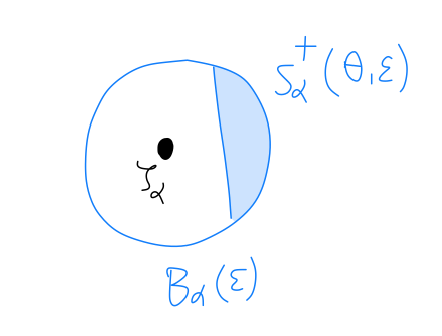
\includegraphics[scale=0.5]{Cattura}
\caption{Representation of $B_\alpha(\varepsilon)$ and the half-moon $S_\alpha^+(\theta,\varepsilon)$.}\label{fig:ball} 
\end{figure}

Then the decomposition is 
\begin{align}\label{decomposition H_B}
H_\bullet(X,zf)=\bigoplus_{\alpha}H_\bullet^{\theta,\alpha}(X,f)
\end{align}     
and the idea of the proof is sketched in Figure \ref{fig:relative_homology}.
\begin{figure}[h]
%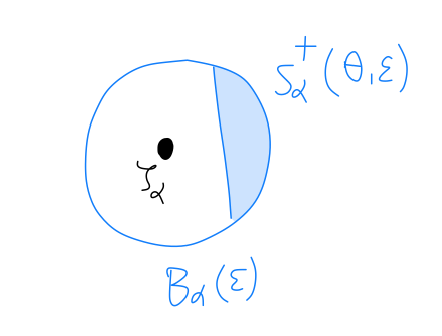
\includegraphics[scale=0.5]{Cattura}
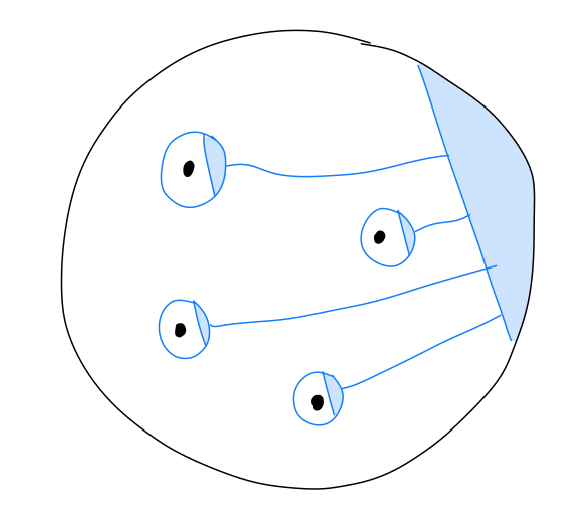
\includegraphics[scale=0.3]{Cattura2}
\caption{Relative homology}\label{fig:relative_homology}
\end{figure}

Let $\theta$ be generic, locally in a neighbourhood of a critcal point $x_\alpha$ we can choose a (real) coordinate system $\xi_1,...,\xi_{2n}$ such that \[e^{i\theta}\left(f(x)-f(x_\alpha)\right)=\sum_{j=1}^n(\xi_j+i\xi_{j+1})^2.\] Then $\mathrm{Re}(e^{i\theta}f)$ is a Morse function with simple, isolated and non degenerate critical points (which are the cirtical points of $f$). We choose a Riemannian metric $g$ on $X$ and we define the \textit{Lefschetz thimbles} $\mathcal{C}_{\alpha,z}$ as the steepstet descendent path issuing from a critcal point $x_\alpha$ (see \cite{Witten}): 
\begin{equation}
\mathcal{C}_{\alpha,z}=\lbrace x=(x_1,...,x_{2n})\in X\,\big\vert \, \lim_{t\to -\infty} x(t)=x_\alpha\rbrace
\end{equation}
where $x(t)$ is the solution of the gradient flow equation \[\frac{\dd x_i(t)}{\dd t}=-g_{ij}\frac{\partial}{\partial \xi_j}\mathrm{Re}f(x(t))\] and $x_i(0)=x_i$ \footnote{An equivalent definition is given by F. Pham in \cite{pham}.}. 

\begin{figure}[h]
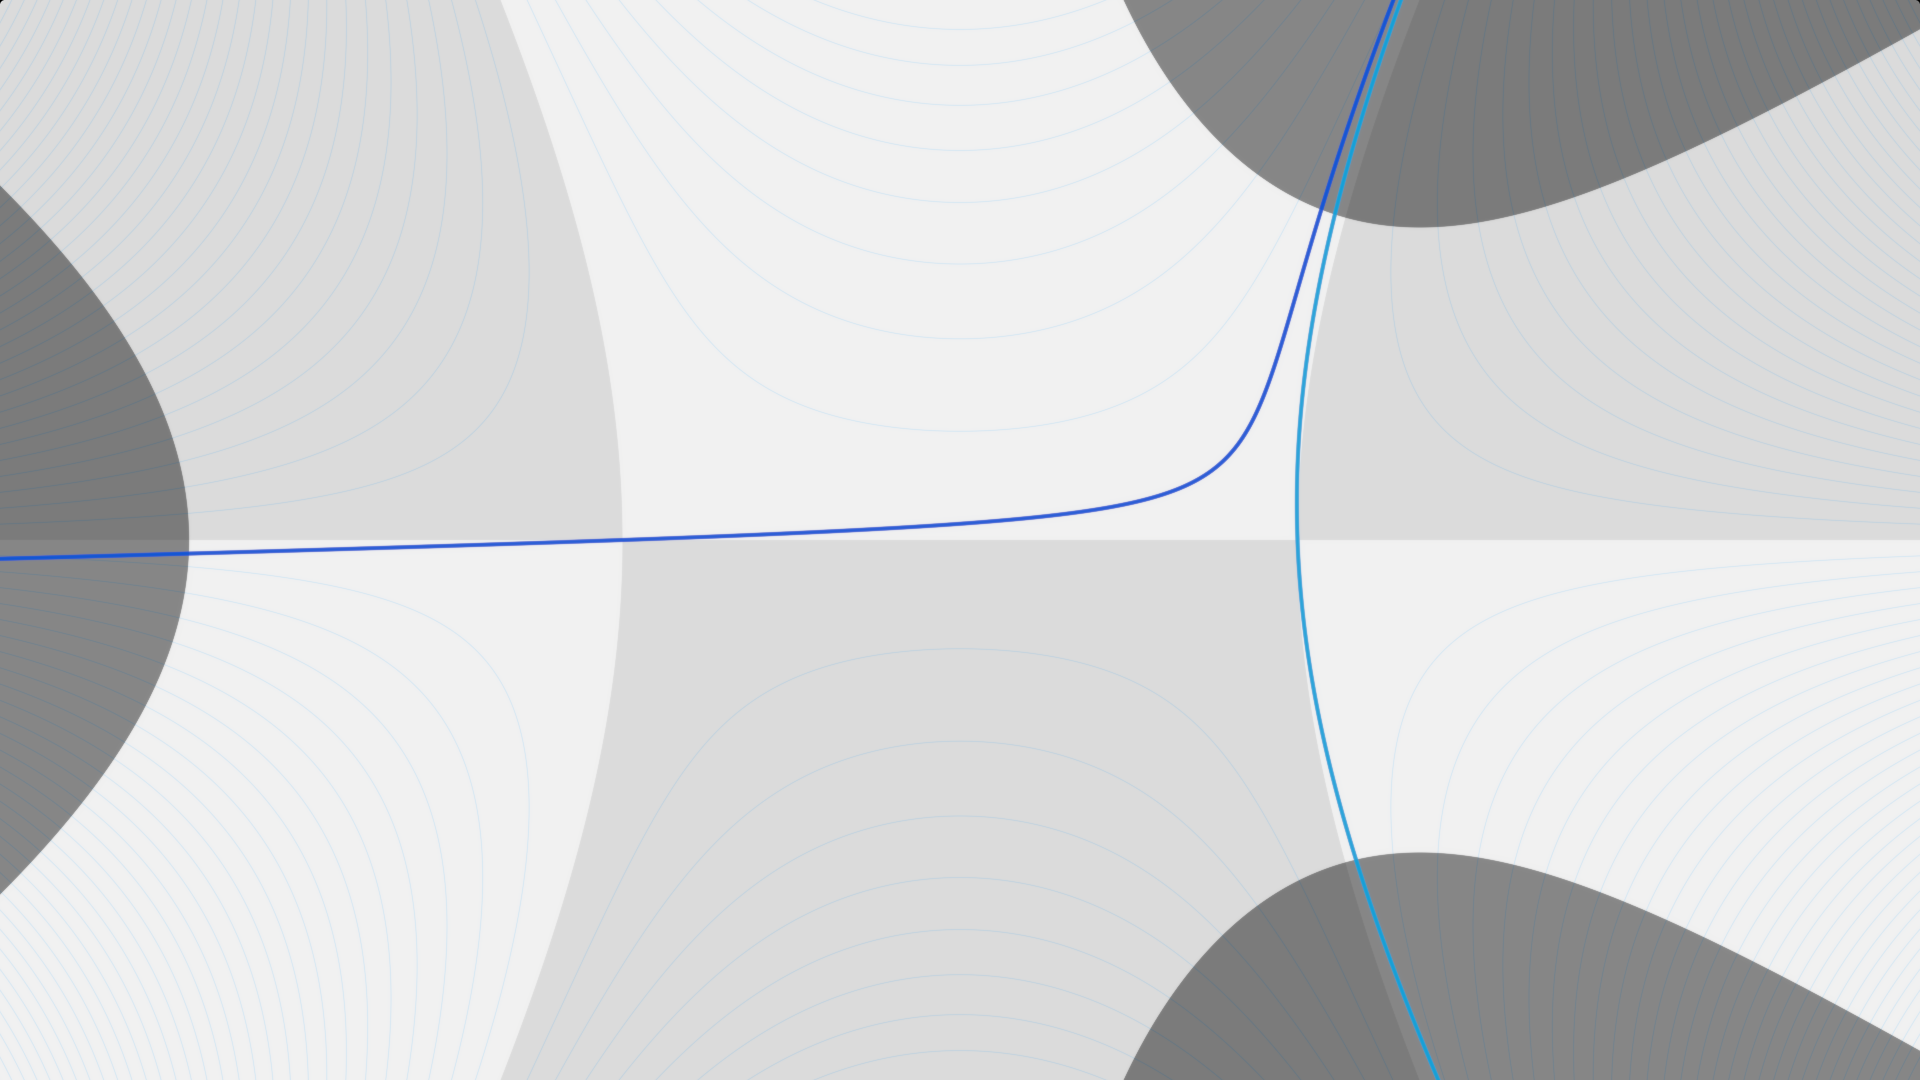
\includegraphics[scale=0.075]{veer-left_matching}
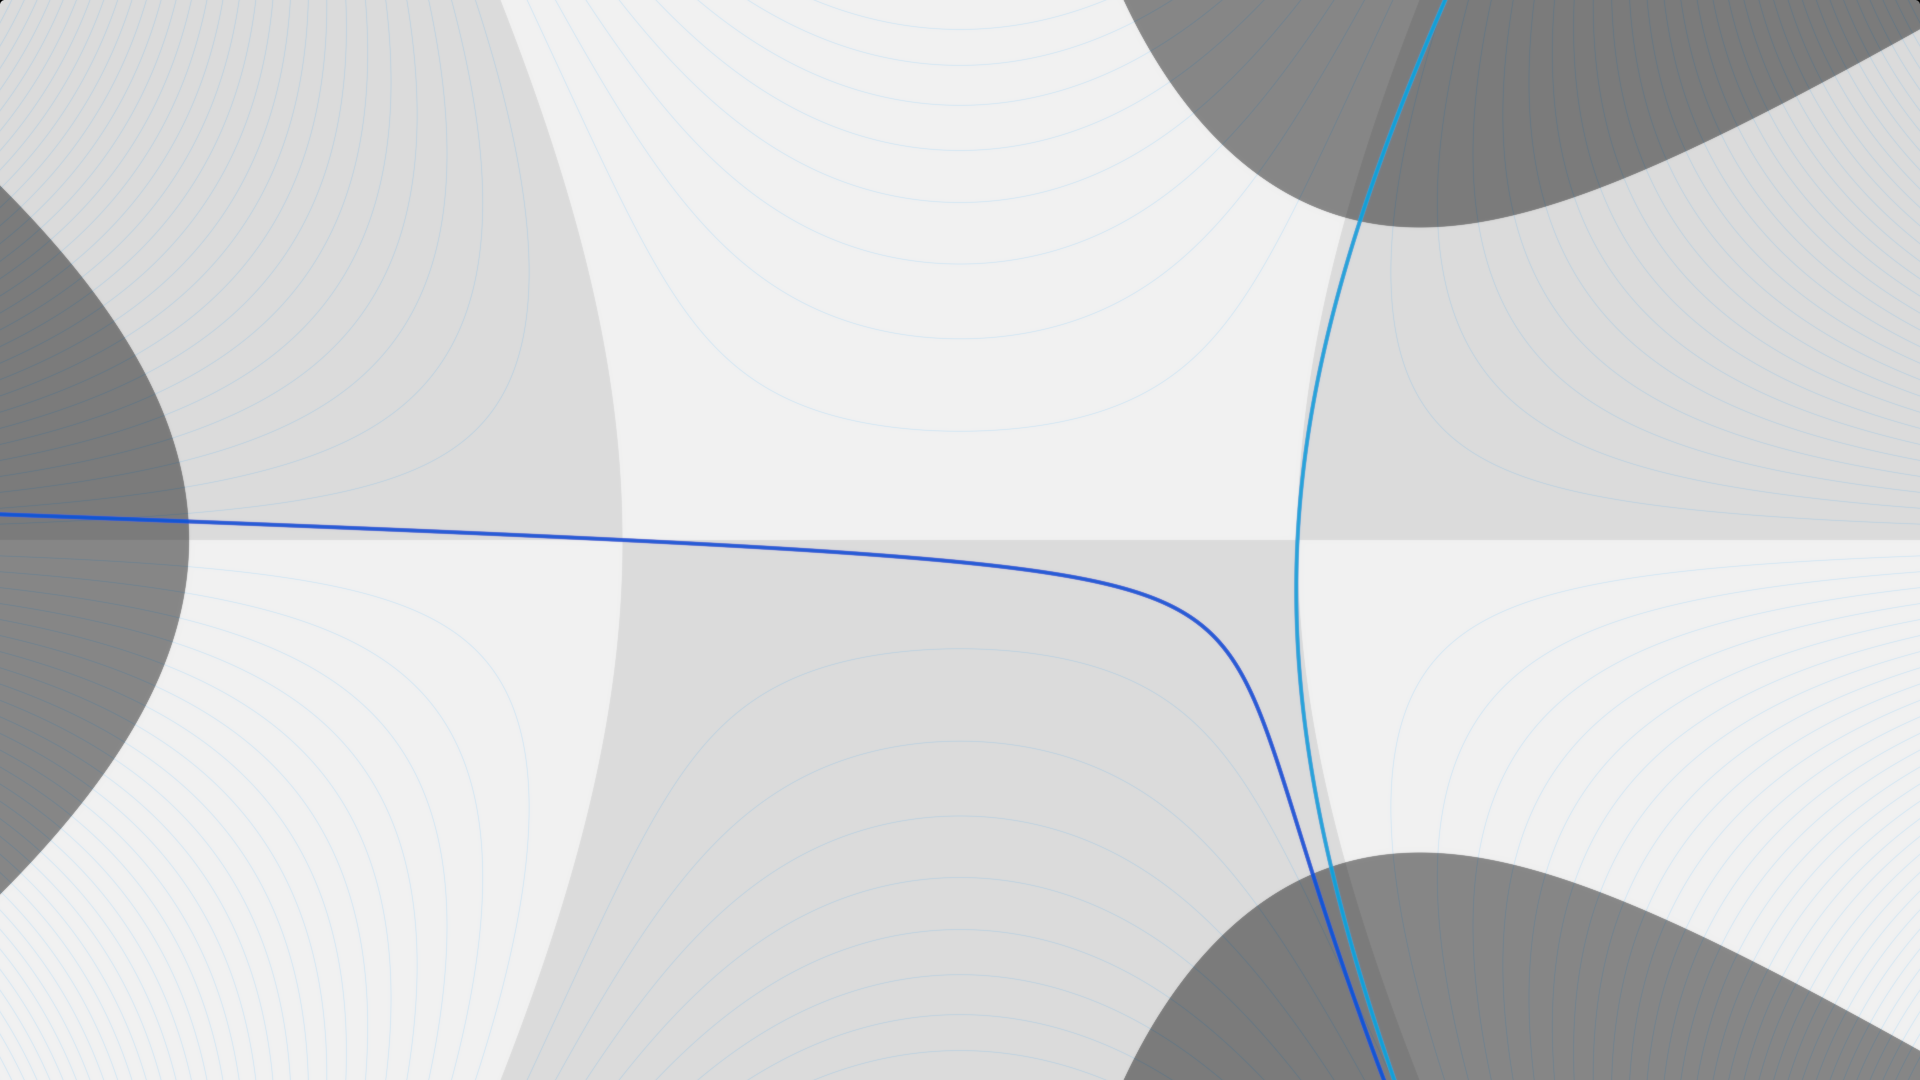
\includegraphics[scale=0.075]{veer-right_matching}
\caption{Lefschetz thimbles for the Airy integral $f(t)=t^3/3-t$ at $\theta=?$ (left) and $\theta=??$ (right). }\label{Lefschetz_thimbles}
\end{figure}

Notice that $[\mathcal{C}_{\alpha,z}]\in H_n(X,zf)$ and they generate the relative homology. In fact,  

\begin{itemize}
\item $H_k^{\theta,\alpha}(X,f)$ is isomorphic to $H_{k-1}(B_\alpha^M(\varepsilon)\cap f^{-1}(\zeta-\zeta_\alpha))$, where $B_\alpha
^M(\varepsilon)$ is an open ball centred at $x_\alpha$ of radius $\varepsilon$ such that for every $\varepsilon'<\varepsilon$ $B_\alpha(\varepsilon')$ is transverse to $f^{-1}(\zeta_\alpha)$. 
\item $H_{k-1}(B_\alpha^M(\varepsilon)\cap f^{-1}(\zeta-\zeta_\alpha))=0$ if $k\neq n$ and $H_{n-1}(B_\alpha^M(\varepsilon)\,\cap f^{-1}(\zeta-\zeta_\alpha))=\Z^\mu$, where $\mu$ is the Milnor number \footnote{The Milnor number counts how many pre-image of a critical value are critical points, or equivalently how many Lefschetz thimbles are in the pre-image of $f^{-1}(\zeta_\alpha+\R_{\geq 0}e^{i\theta})$.};   
\end{itemize}

hence $H_n^{\theta,\alpha}(X,f)$ has rank $\mu$. In addition from singularity theory we know that the set of vanishing cycles $\partial\mathcal{C}_{\alpha,z}$ forms a basis of $H_{n-1}(B_\alpha^M(\varepsilon)\cap f^{-1}(\zeta-\zeta_\alpha)) $ (see Theorem 2.1 \cite{Arnold}).    

  
Since for $\theta$ generic the collection of the Lefschetz thimbles $\mathcal{C}_{\alpha,z}\in H_n^{\theta,\alpha}(X,f)$ (for all $\alpha$ and fixed $\theta$)are a basis for the relative homology $H_n(X,zf)$, the integral $I(z)$ can be decomposed as sum over Lefschetz thimbles: we denote 
\begin{equation}\label{int_alpha}
I_{\alpha}(z)\defeq\int_{\mathcal{C}_{\alpha,z}}e^{-zf}\nu
\end{equation}
and we refer to $I_{\alpha}(z)$ as a thimble integral. Then  for every $[\mathcal{C}]\in H_n(X,zf)$
\begin{align*}
I(z)=\sum_{\alpha}n_\alpha I_{\alpha}(z). 
\end{align*}
Moreover the coeficients $n_\alpha$ can be computed via intersection theory (see $\S 5$ \cite{pham}, $\S 3.1.5$ \cite{Witten}). When $X$ is not compact the intersection paring is defined introducing dual cycles: let 
\begin{align*}
\mathcal{K}_{\alpha,z}\defeq\lbrace x\in X\,\big\vert\, \lim_{t\to -\infty} x(t)=x_\alpha \rbrace
\end{align*} 
where $x(t)$ solve the upward flow equation
\begin{align*}
\frac{\dd x_i(t)}{\dd t}= g_{ij}\frac{\partial}{\partial \xi_j}\mathrm{Re}f(x(t)) \qquad \text{ with } x_i(0)=x_i
\end{align*}
then $\mathcal{K}_{\alpha,z}\in H_{n}(X,f^{-1}(S^-_c);\Z)$ for $c$ large enough and they define a basis (for $\theta$ generic). Furthermore, $\mathcal{K}_{\alpha,z}$ and $\mathcal{C}_{\alpha,z}$ intersect transversely at the critical point $x_\alpha$, hence they define a non degenerate pairing 
\begin{align*}
\langle -, -\rangle\colon H_n&(X,f^{-1}(S^+_c);\Z)\otimes H_n(X,f^{-1}(S^-_c);\Z)\to \Z \\
& \qquad \mathcal{C} \qquad\quad , \qquad\qquad \mathcal{K} \qquad \to \quad \langle\mathcal{C} , \, \mathcal{K}\rangle. 
\end{align*}
\color{magenta}
Should I mention the Betti--DeRham iso? 

\color{black}


Now looking at the intersection of $\mathcal{C}\in H_n(X,zf)$ with the basis $\mathcal{K}_{\alpha,z}$ we can compute the constants $n_\alpha$ in terms of intersection pairing:
\begin{align*}
\langle \mathcal{C},\mathcal{K}_{\alpha,z}\rangle=\langle \sum_\beta n_\beta\mathcal{C}_{\beta,z},\mathcal{K}_{\alpha,z}\rangle=\sum_{\beta}n_\beta\langle \mathcal{C}_{\beta,z},\mathcal{K}_{\alpha,z}\rangle=\sum_{\beta}n_\beta\delta_{\alpha\beta}=n_\alpha
\end{align*}

hence $n_\alpha$ are integers. However, there are examples in which $n_\alpha\in\C$ (see modified Bessel): indeed if there exists a group $G$ that leaves $f$ invariant, namely
\begin{align*}
f(g.x)=f(x)\,\,\forall g\in G
\end{align*} 
then different critical points can be mapped to the same critical value. It follows that for every $x_j$ in the orbit of $x_\alpha$, the thimbles $\mathcal{C}_{j,z}=f^{-1}(\zeta_\alpha+ \R_{\geq 0} e^{i\theta})$ are $\C$-linear dependent.
 
% $H_\bullet(X,zf)$ such that the orbits of $\mathcal{C}_{\alpha,z}\in H_n^{\theta,\alpha}(X,f)$ contains the Lefschetz thimbles $\mathcal{C}_{j,z}\in H_n^{\theta,z}(X,zf)$ for every $j$ such that $f(x_j)=\zeta_\alpha$. When it happens, $\mathcal{C}_{j,z}$ and $\mathcal{C}_{\alpha,z}$ are $\C$- linear dependent, hence the coefficients $n_j$ are complex valued. 


\color{magenta}
ORIENTATION? 

$n_\alpha=(-1)^{n(n-1)/2}\langle \mathcal{C}_{\alpha,\theta+\pi},\mathcal{C}\rangle$ 

\color{black}

\subsection{Borel regularity}

Borel resummation is a way of turning a formal power series
\[ \series{\varphi} = z^\sigma \left( \frac{\varphi_0}{z} + \frac{\varphi_1}{z^2} + \frac{\varphi_2}{z^3} + \frac{\varphi_3}{z^4} + \ldots \right), \]
with $\sigma \in [0, 1)$, into a function which is asymptotic to $\series{\varphi}$ as $z \to \infty$. Different functions can be asymptotic to the same power series, and Borel resummation picks one of them, performing an implicit regularization~\textbf{[arXiv:1705.03071, or maybe arXiv:1412.6614]}. When a function matches the Borel sum of its asymptotic series, we'll say it's {\em Borel regular}. Several familiar kinds of regularity imply Borel regularity, and shed light on why it occurs.
%%Knowing that a function is Borel regular gives us extra information about it---enough to reconstruct it from its asymptotic series. What's the nature of this extra information?
%%Since different functions can be asymptotic to the same power series, Borel resummation must involve an {\em implicit regularization}, restricting its range to a class of functions which are uniquely determined by their formal power series.
\begin{itemize}
\item \textbf{Having a good asymptotic approximation}

Let $R_N$ be the difference between a function and the partial sum
\[ \frac{\varphi_0}{z} + \frac{\varphi_1}{z^2} + \frac{\varphi_2}{z^3} + \ldots + \frac{\varphi_{N-2}}{z^{N-1}} \]
of its asymptotic series. Watson showed a century ago that the function is Borel regular whenever there's a constant $c \in (0, \infty)$ with
\[ |R_N| \le \frac{c^{N+1} N!}{|z|^N} \]
over all orders $N$ and all $z$ in a wide enough wedge around infinity.
\item \textbf{Satisfying a singular differential equation}

\begin{itemize}
\item Think about conditions where this works.
\item Maybe the correct place is the setting of Ecalle's formal integral. See \S 5.2.2.1 of Delabaere's {\em Divergent Series, Summability and Resurgence III}.
\item Say there's a unique solution (up to scaling) that shrinks as you go right; everything else blows up exponentially. Then this is the only solution that can be expressed as a Laplace transform.
\item If the Borel-transformed equation has a subexponential solution $\hat{f}$ which is ``shifted holomorphic'' (we called this having a ``fractional power singularity'' in {\tt airy-resurgence}), then $\laplace \hat{f}$ satisfies the original equation, because there are no boundary terms.
\item Draw diagram showing formal vs. holomorphic solutions in time vs. frequency domains.
\end{itemize}
\item \textbf{Being a thimble integral}

Under the previous assumptions, we can now state a Borel regularity result for thimble integrals: 
 
\begin{theorem}\label{thm:borel integrals}
Borel regularity for thimbles integrals can be stated a the commutativity of the following diagram:
\begin{equation}
\begin{tikzcd}
I_{\alpha}(z)\defeq\int_{\mathcal{C}_\alpha}e^{-zf}\nu \arrow[r,"\sim"]\arrow[dd, swap, "\mathcal{L}^\theta "] & \tilde{I}_{\alpha}(z)\arrow[dd,"\mathcal{B}"]\\
& \\
\hat{\iota}_\alpha(\zeta)\arrow[r,equal,swap, "\text{sum}"] & \tilde{\iota}_{\alpha}(\zeta) 
\end{tikzcd}
\end{equation}
\end{theorem}

A priori, the Laplace transform of $\hat{\iota}_\alpha(\zeta)$ and $I_{\alpha}(z)$ have the same asymptotic behaviour in a given sector (indeed taking the asymptotic of $I_\alpha(z)$ we \textit{loose} information); however Borel regularity guarantees that $I_{\alpha}(z)=\mathcal{L}^{\theta}\hat{\iota}_{\alpha}$ in a given sector. We give a proof of Theorem \ref{thm:borel integrals} in Section ?? \ref{thm:maxim} when $N=1$, and the proof is based on the fact that $I_\alpha(z)$ can be rewritten as the Laplace transform--type integral. In higher dimension the same result was stated in \cite{Dunne-Unsal 15} (but the proof was not written).

Generically, $\tilde{I}_{\alpha}(z)$ is a divergent series whose coefficients factorially grow and, as proved by Berry and Howls \cite{BH}\cite{H} the divergence of $\tilde{I}_{\alpha}(z)$ encodes contributions from the other critical points of $f$ in the form of \textit{exact resurgence relation} (see equation 19 \cite{BH}). Indeed, the Borel transform $\hat{\iota}_\alpha(\zeta)$ yet contains information about the Borel transform $\hat{\iota}_{\beta}(\zeta)$ at other critical values $\zeta_\beta$. This is the idea of resurgence of $\tilde{I}_{\alpha}(z)$ \cite{EcalleI}\cite{EcalleII}\cite{EcalleIII}. However, since $f$ has finitely many critical points and $\nu$ is meromorphic, Borel--Laplace summability properties and resurgence of exponential integrals are straightforward. However, in order to completely describe the Borel plane one needs to compute the Stokes data which provide the analytic continuation across the branch cut. In particular for a certain class of exponential integrals the analytic theory developed by J. Ecalle to compute the Stokes data (see \cite{Ecalle}\cite{diverg-resurg-i}\cite{Dorigoni}\cite{Schiappa}) has a geometric interpretation relying on intersection theory of dual relative homology classes in the sense of F. Pham \cite{pham} (see also \cite{Maxim_lectures}\cite{Maxim_slide_ERC}).   
\end{itemize}


\subsection{Stokes phenomena for exponential integrals}
So far we have considered $\theta=\arg(z)$ fixed and generic (i.e. $\theta\neq\arg(\zeta_\alpha-\zeta_\beta)$), but as we let $\theta$ varying $I_{\alpha}(z)$ becomes a multivalued function. Indeed when $\theta$ crosses a Stokes ray $\ell_{\alpha\beta}\defeq\arg(\zeta_\alpha-\zeta_\beta)\R$, $I_\alpha(z)$ jumps. Computing the jumps of $I_{\alpha}(z)$ is equivalent to determine the analytic continuation of $I_\alpha(z)$ for $z\in\C$. There are different ways to compute the Stokes jumps across the rays $\ell_{\alpha\beta}$: one is purely geometric, based on the way the decomposition \eqref{decomposition H_B} varies as $\theta$ varies. Another one is based on the resurgence analysis of the asymptotic expansion of $I_{\alpha}(z)$ as $\mathrm{Re}(z e^{i\theta})\to +\infty$. In Section \ref{sec:Stokes} we prove that the geometric and the resurgence approach to compute the Stokes jumps are equivalent:
\begin{theorem}[Theorem \ref{Stokes}]

\end{theorem}  

    
\subsubsection{Geometric computation of Stokes constants}
As we discuss in $\S$\ref{what-are-exp-inte}, at $\theta$ generic, the relative homology groups $H_n(X,zf)$ admits a decomposition in terms of the homology relative to each critical values $H_n^{\theta,\alpha}(X,f)$. As $\theta$ varies, $H_n^{\theta,\alpha}(X,f)$ defines a rank $\mu$ local system over $\mathbb{S}^1$ which has non trivial monodromy at the singular points $\theta=\arg(\zeta_\alpha-\zeta_\beta)$. Our goal is to compute these monodromy matrices: on a Stokes ray $\ell_{\alpha\beta}=\zeta_\alpha+e^{i\theta}\R$ the imaginary part of $\zeta_j\in\ell_{\alpha\beta}$ is constant and we order the critical values as $\mathrm{Re}(\zeta_1)<\mathrm{Re}(\zeta_2)<...<\mathrm{Re}(\zeta_j)$. Then the monodromy matrices are upper triangular and the off diagonal terms are the so called Stokes constants. 
In order to compute the Stokes constants we follow Kontsevich's proposal in \cite{Maxim_lectures} which is in terms of intersection numbers of thimbles. 


\begin{figure}[h]
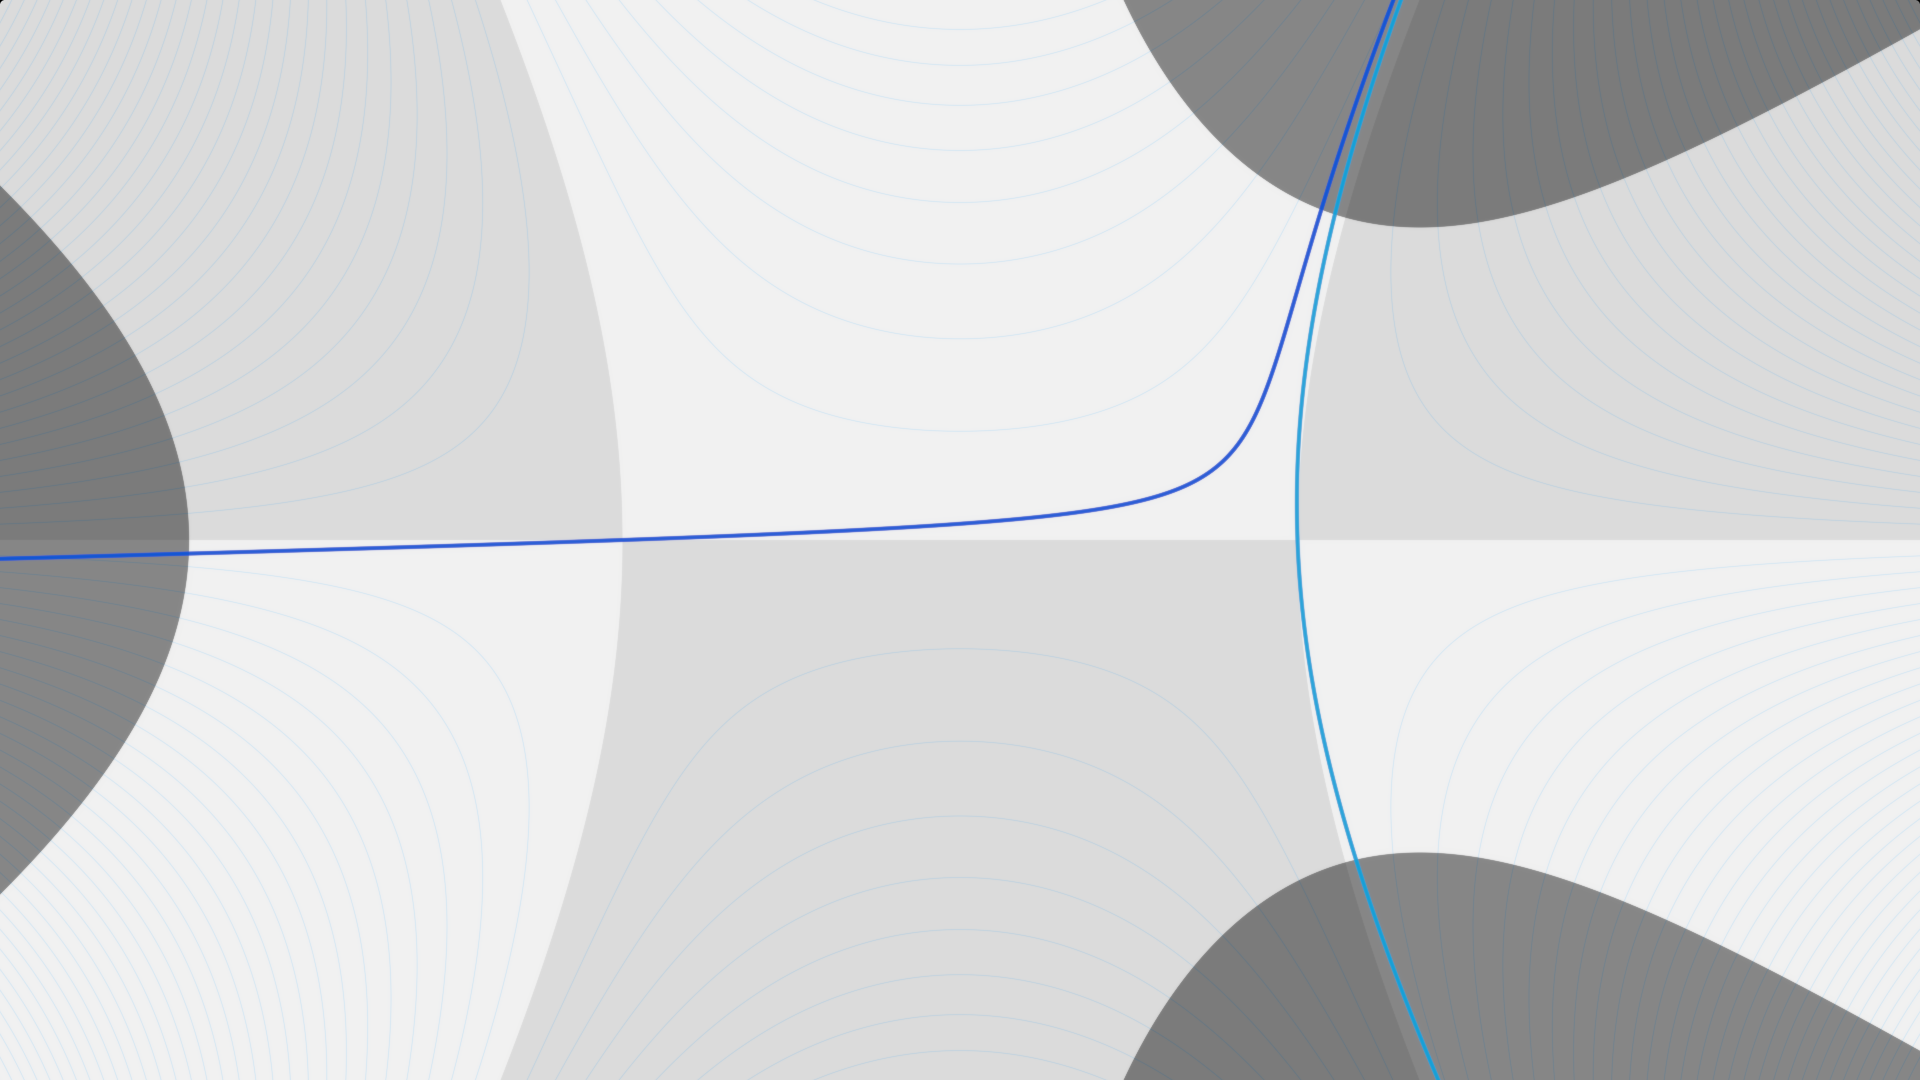
\includegraphics[scale=0.065]{veer-left_matching}
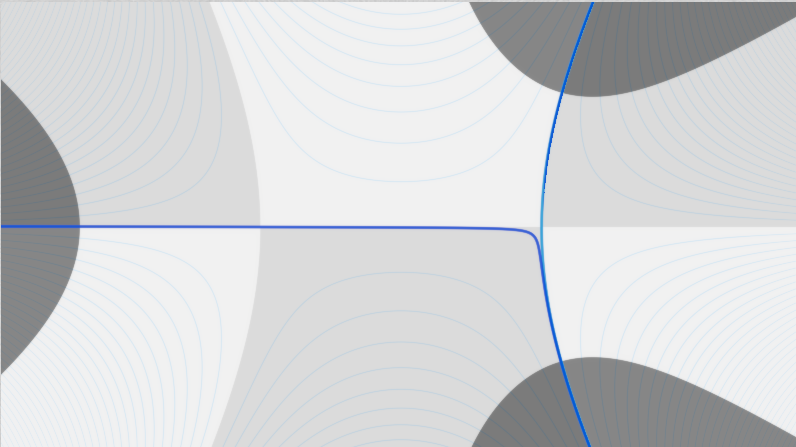
\includegraphics[scale=0.26]{thimble-degenerate}
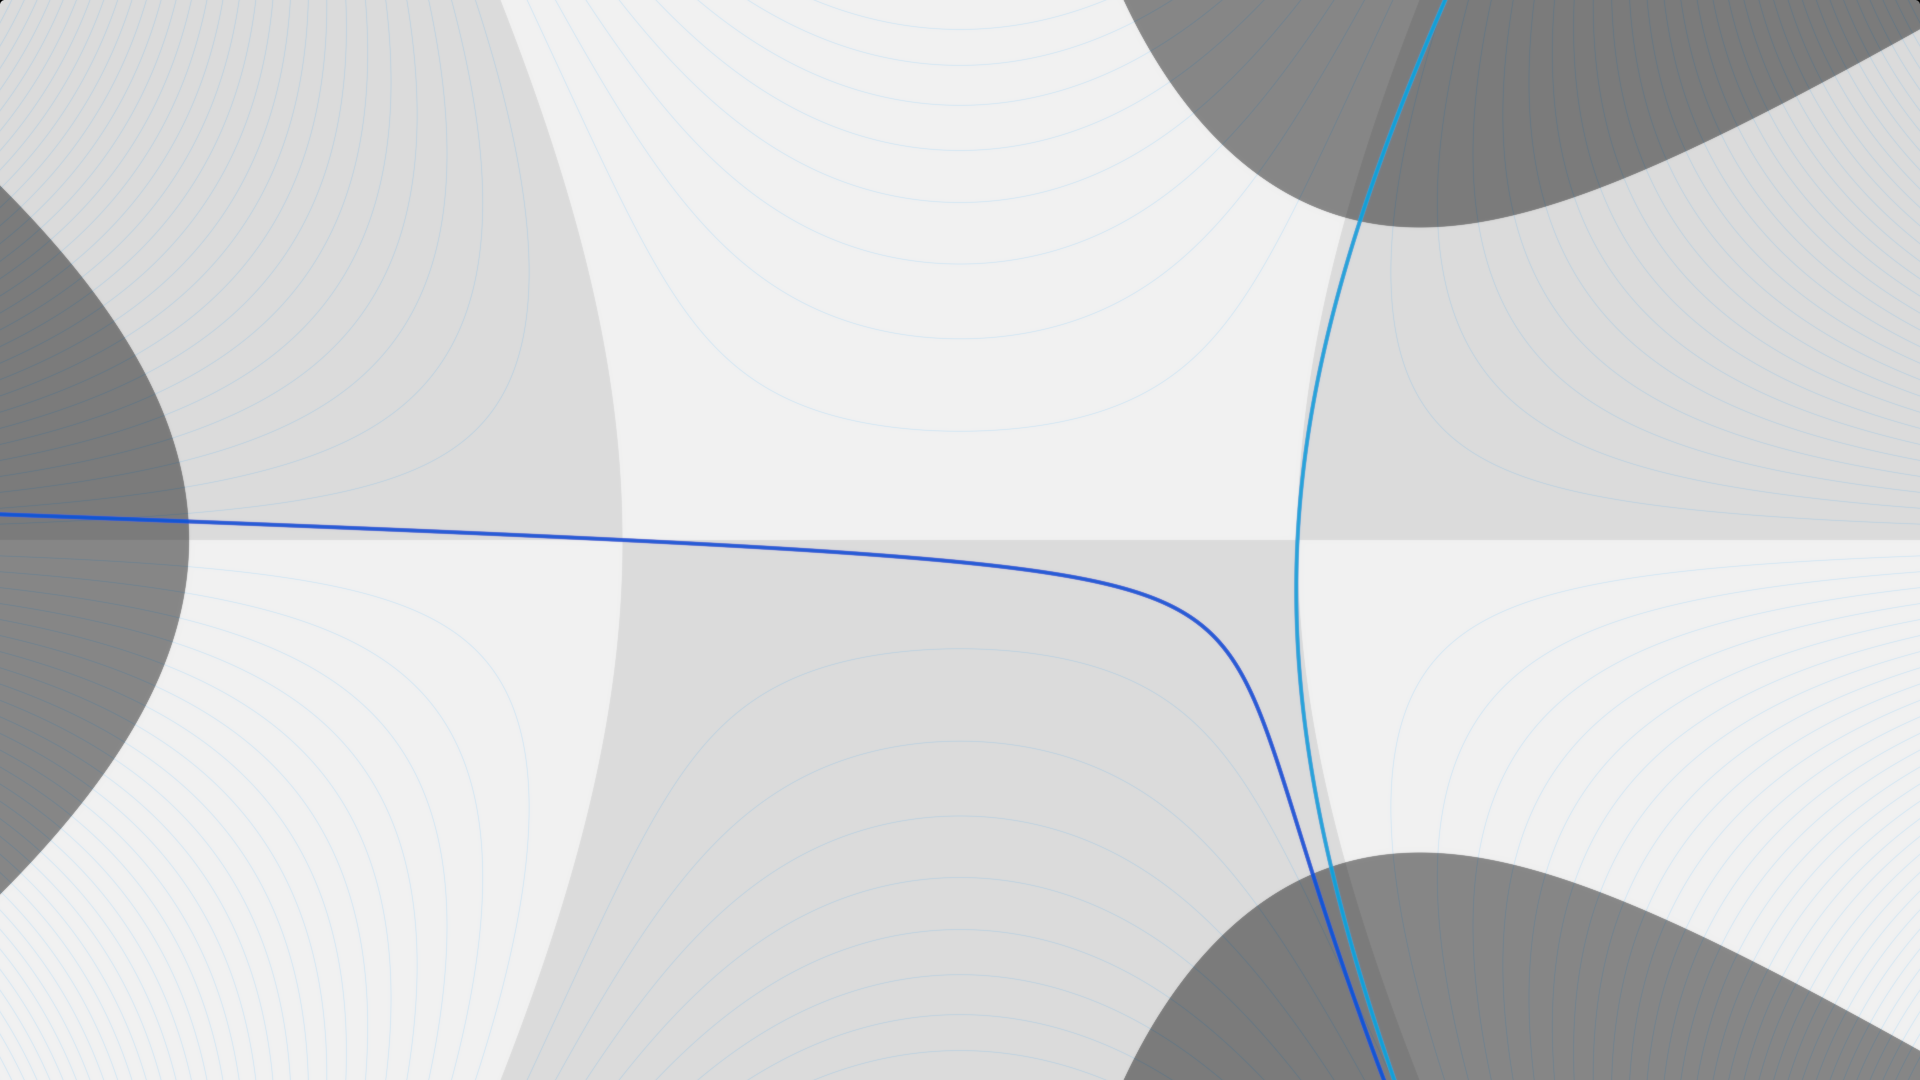
\includegraphics[scale=0.065]{veer-right_matching}
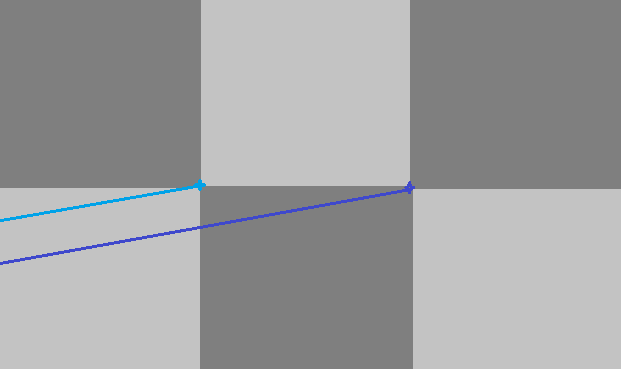
\includegraphics[scale=0.33]{borel-left}
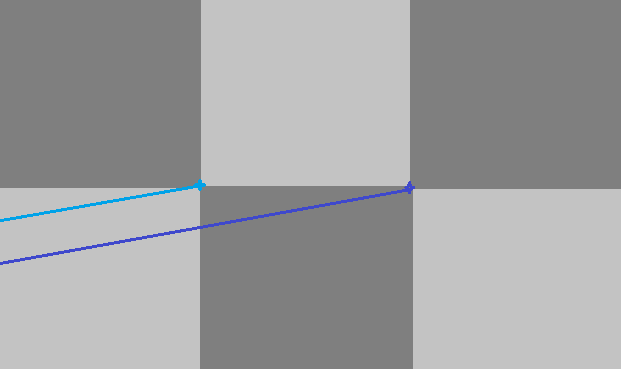
\includegraphics[scale=0.33]{borel-left}
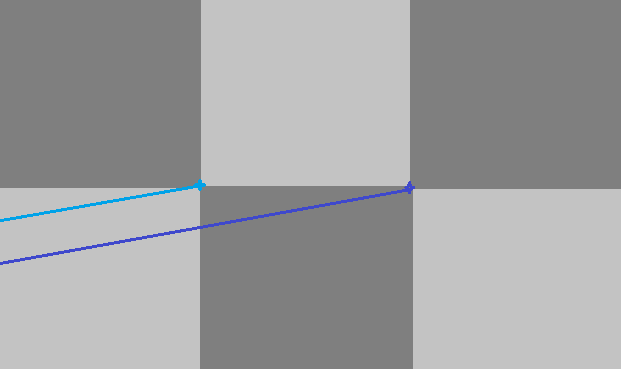
\includegraphics[scale=0.33]{borel-left}
\end{figure}    


\subsubsection{ ODE and fractional derivative formula [draft2]}

From an analytic perspective, Stokes phenomena occurs studying the analytic continuation of germs of holomorphic function in the Borel plane. Indeed, Borel transform of divergent series usually have singularities and the aim of resurgence theory is to investigate the analytic continuation away from the singularities. We will mainly refer to J. Ecalle's orginal papers \cite{EcalleI}\cite{EcalleII}\cite{EcalleIII} as well as the following introductive reviews by different authors \cite{Schiappa}\cite{Dorigoni}\cite{diablerets}\cite{MS16}\cite{sauzin_Gamma}.  

Among the most common type of singularities of $\hat{\iota}(\zeta)\in\C\lbrace\zeta\rbrace$ there are simple singularities and fractional power singularities: 
\begin{itemize}
\item $\hat{\iota}(\zeta)$ has a simple singularity at $\omega\in\C$ if there exist a constant $C_\omega\in\C$ and a germ of holomorphic function at the origin $\hat{\phi}_\omega(\zeta)\in\C\lbrace\zeta\rbrace$ such that in a neighbourhood of $\omega$
\begin{align*}
\hat{\iota}(\zeta-\omega)=\frac{C_\omega}{2\pi i \zeta}+\frac{\mathrm{Log}(\zeta)}{2\pi i}\hat{\phi}_{\omega}(\zeta)+\text{ hol. fct.}
\end{align*} 
and $\mathrm{Log}(\zeta)$ is any branch of the logarithm;
\item $\hat{\iota}(\zeta)$ has a fractional power singularity at $\omega\in\C$ if there exist $\mu\in\Q\setminus\Z$ and a germ of holomorphic function at the origin $\hat{\phi}_\omega(\zeta)\in\C\lbrace\zeta\rbrace$ such that in a neighbourhood of $\omega$
\begin{align*}
\hat{\iota}(\zeta-\omega)=\zeta^{\mu}\hat{\phi}_\omega(\zeta)+ \text{ hol. fct.}
\end{align*}
\end{itemize} 

From the type of singularities we can study the analytic continuation of $\hat{\iota}$; for instance in both the previous examples we look for singularities of the germ $\hat{\phi}_\omega(\zeta)$ iterating the same procedure. In general, this iterative procedure may be infinite as at every step we may found new singularities, however resurgence function are endlessly analytic continuable, meaning that at each step they admit only finitely many singularities. There are also examples where the resurgence structure of germs is easier because there are only finitely many singularities, as it happens for exponential integrals and for solutions of linear ODEs. In particular, in the former case the singularities are the critical values of the potential $f$ while in the latter they are determined from the equation written in the \textit{prepared form}. In both cases the singularities are fractional power singularities but for exponential integrals (as a corollary of Theorem \ref{thm:borel integrals}) we will prove a fractional derivative formula which expresses the non-fractional singularity $\hat{\varphi}_\alpha(\zeta)$ in terms of the Borel transform  $\hat{\iota}_\alpha(\zeta)$:

\begin{corollary}[see Corollary \ref{int:deriv-formula}]\label{cor:deriv-formula} 
Under the same assumptions of Theorem \ref{thm:borel integrals}, for any $\zeta$ on the ray going rightward from $\zeta_\alpha$ in the direction of $\theta$, we have
\begin{multline}
\hat{\varphi}_{\alpha}(\zeta)=\partial^{3/2}_{\zeta \text{ from }\zeta_\alpha} \left( \int_{\mathcal{C}_\alpha(\zeta)}\nu \right)={\left(\tfrac{\partial}{\partial \zeta}\right)^2}\,\frac{1}{\Gamma\big(\tfrac{1}{2}\big)} \int_{\zeta_\alpha}^\zeta (\zeta-\zeta')^{-1/2} {\left( \int_{\mathcal{C}_\alpha(\zeta')} \nu \right)}\,d\zeta',
\end{multline}
where $\mathcal{C}_\alpha(\zeta)$ is the part of $\mathcal{C}_\alpha$ that goes through $e^{-i\theta}f^{-1}([\zeta_\alpha, \zeta ])$. Notice that $\mathcal{C}_\alpha(\zeta)$ starts and ends in $e^{-i\theta}f^{-1}(\zeta)$. 
\end{corollary}

Conjecturally, we expect $\hat{\varphi}_\alpha(\zeta)$ to have simple singularities. Moreover, in the examples, $\hat{\varphi}_\alpha(\zeta)$ turn out be an hypergeometric function of type ${}_pF_{p-1}$ where $p$ is the number of critical values. 
We expect that hypergeometric functions play a special role in resurgence theory as they may always appear when there are only finitely many singularities. In addition,  \textbf{Aaron-> what do you expect to be true in terms of the algebraic hypergeometric?} 


%Another difficulty of studying the analytic continuation of a germ is that often we only know its series expansion $\tilde{\iota}(\zeta)$ and not its sum $\hat{\iota}(\zeta)$ which  

Once we know the location of singularities hence the analytic continuation of the germ, the Stokes constant are determined either by comparing the behaviour across a branch cut or the residue at a simple pole. We discuss the two cases separately: let $\hat{\iota}(\zeta)\in\C\lbrace\zeta\rbrace$ be a germ at the origin with a log singularity at $\omega\in\C$

\begin{equation}
\hat{\iota}(\zeta-\omega)=\frac{\mathrm{Log}(\zeta)}{2\pi i}\hat{\phi}_{\omega}(\zeta)+\text{ hol. fct.}
\end{equation} 

with $\hat{\phi}_{\omega}(\zeta)\in\C\lbrace\zeta\rbrace$. If  $\hat{\phi}_{\omega}(\zeta)$ has no singularities for $\mathrm{Re}(\zeta)\geq \mathrm{Re}(\omega)$, then $\hat{\iota}$ has a branch cut for $\zeta=\omega+\R_{\geq 0}$  and its analytic continuation is easily computed

\begin{align*}
\hat{\iota}(\zeta-\omega+i\epsilon)-\hat{\iota}(\zeta-\omega-i\epsilon)&=\frac{\mathrm{Log}(\zeta+i\epsilon)}{2\pi i}\hat{\phi}_\omega(\zeta+i\epsilon)-\frac{\mathrm{Log}(\zeta-i\epsilon)}{2\pi i}\hat{\phi}_\omega(\zeta-i\epsilon)\\
&=\frac{\mathrm{Log}(\zeta-i\epsilon)+2\pi i}{2\pi i}\hat{\phi}_\omega(\zeta)-\frac{\mathrm{Log}(\zeta-i\epsilon)}{2\pi i}\hat{\phi}_\omega(\zeta)\\
&=\hat{\phi}_\omega(\zeta). 
\end{align*} 
We can deduce that the log singularity is represented by $\hat{\phi}_{\omega}(\zeta)$ also called \textit{minor} in Ecalle formalism. 

Similarly, if $\hat{\iota}$ has fractional power singularity $\mu\in\C\setminus\Z$ and $\hat{\phi}_{\omega}$ has no singularities in $\omega+\R_{\geq 0}$, across the branch cut $\omega+\R_{\geq 0}$ 

\begin{align*}
\hat{\iota}(\zeta-\omega+i\epsilon)-\hat{\iota}(\zeta-\omega-i\epsilon)&=(\zeta+i\epsilon)^{\mu}\hat{\phi}_\omega(\zeta+i\epsilon)- (\zeta-i\epsilon)^{\mu}\hat{\phi}_\omega(\zeta-i\epsilon)\\
&=e^{2\pi i\mu}(\zeta-i\epsilon)^\mu\hat{\phi}_\omega(\zeta)-(\zeta-i\epsilon)^{\mu}\hat{\phi}_\omega(\zeta)\\
&=(e^{2\pi i\mu}-1)(\zeta-i\epsilon)^{\mu}\hat{\phi}_{\omega}(\zeta).
\end{align*} 
In this case, a \textit{minor} is given by $(e^{2\pi i\mu}-1)(\zeta-i\epsilon)^{\mu}\hat{\phi}_{\omega}(\zeta)$. 

In Ecalle formalism, pole singularities are usually denoted by the symbol $\delta^{(k)}$ where $k$ represent the order of the pole:
\begin{align*}
\delta\defeq\mathrm{sing}_0\left(\frac{1}{2\pi i\zeta}\right) \qquad\qquad \delta^{(k)}\defeq\mathrm{sing}_0\left(\frac{(-1)^kk!}{2\pi i\zeta^{k+1}}\right),\quad k\geq 0
\end{align*}
where $\mathrm{sing}_0$ denotes the quotient map by germs of holomorphic functions. According to that notation, simple singularities are denoted by 
\begin{equation}
\overset{\triangledown}\iota(\zeta)=C_\omega\delta+\hat{\varphi}_{\omega}(\zeta).
\end{equation}  

\color{green}

parla Stokes constant in generale

\color{black}

Let us focus on the Stokes phenomena for exponential integrals: let $\zeta_{\alpha_i}$, $i=1,...,N$ be the critical values of $f$ and $x_1,...,x_d$ be the critical points (where $d$ might be grater than $N$). For each critical point, the asymptotic behaviour of $I_{j}(z)$ is given by a formal power series $\tilde{I}_{j}(z)$ whose Borel transform is a germ of holomorphic functions at $f(x_j)=\zeta_{\alpha_i}$ for some $i$. In addition, $\hat{\iota}_{j}(\zeta)$ has singularities in the Borel plane exactly at points $\zeta_{\alpha_l}$ for $l\neq i$. Hence, if we define $R_{jk}\defeq |\zeta_{\alpha_i}-\zeta_{\alpha_l}|$ for $k$ such that $f(x_k)=\zeta_{\alpha_l}$ and we order $\zeta_{\alpha_l}$ so that $R_{jk_1}\leq R_{jk_2}\leq ...\leq R_{jk_N}$ in a neighbourhood of $\zeta_{\alpha_l}$ we expect  

\begin{equation}
\hat{\iota}_j(\zeta-\zeta_{\alpha_l})=\sum_{r: R_{jk_1}=R_{jk_r}}S_{jk_r}\hat{\iota}_{k_r}(\zeta) 
\end{equation}  
where $S_{jk}$ are constants. Notice that there might be more values of $k$ such that $f(x_k)=\zeta_{\alpha_l}$ for a fixed $l$; hence the constants $S_{jk}$ are defined only after a choice of normalization. \textbf{Discuss with Aaron what is the best choice; should we fix a basis of critical points and relate the thimbles with the same image via the action of some group? How this affect the constants?}   


Going back to the $z-$ plane, from the analysis on the Borel plane we deduce the following: let ...

we can also compute the Stokes constants via direct computation of the analytic continuation of the Borel--Laplace sum of $\tilde{I}_{j}(z)$ for every $j$ such that $\zeta_j\in\ell_{\alpha\beta}$. This is about computing the difference between $\mathcal{L}_{\theta_\pm}\hat{\iota}_{j}\defeq\int_{ 
\zeta_j}^{e^{i\theta_\pm}\infty}e^{-z\zeta}\hat{\iota}_{j}(\zeta)d\zeta$ such that $\theta_\pm=\arg(\zeta_\alpha-\zeta_\beta)\pm\epsilon$, $\epsilon <\!\!< 1$ does not contain other singularities of $\hat{\iota}_j(\zeta)$. Following the convention of \cite{Dorigoni}\cite{Schiappa} we define the Stokes automorphisms $\mathfrak{S}_\theta$ associated to the critical direction $\theta$ as 

\begin{align*}
\mathcal{L}_{\theta_+}=\mathcal{L}_{\theta_-}\circ\mathfrak{S}_{\theta}
\end{align*}
which measures the jump between the Borel--Laplace sum of $\tilde{I}_j(z)$ across the ray $\ell_{\alpha\beta}$. In addition it can be expressed in terms of the so called \textit{Alien derivatives} $\Delta_{\zeta_{j}}$ for every $\zeta_{j}\in\ell_{\alpha\beta}$ which are derivations on the algebra of resurgent functions

\begin{align*}
\Delta_{\zeta_j}\colon 
\end{align*} 

in particular, if $\hat{\iota}_j(\zeta)$ is a resurgent function 
Then 

\begin{align*}
\mathfrak{S}_{\theta}= \exp\left(\right)
\end{align*}



\subsubsection{If hypergeometric functions appear in a large class of examples: integral formulas for hypergeometric functions }

\subsection{Plan of the paper}

\section{Formalism of the Laplace transform}

\section{Borel regularity}

\subsection{ODEs}

\subsection{Thimble integrals}
We are going to prove Theorem \ref{thm:borel integrals}. 
Let $X$ be a $n$-dimensional algebraic variety, $f\colon X\to\C$ be an algebraic function with simple, isolated, non-degenerate critical points, and $\nu\in\Gamma(X,\Omega^n)$, and we consider
\begin{equation}
I_{\alpha}(z)\defeq\int_{\mathcal{C}_\alpha}e^{-zf}\nu
\end{equation}
where $\mathcal{C}_{\alpha,z}$ is a Lefschetz thimble $[\mathcal{C}_{\alpha,z}]\in H_n(X,zf)$ for $\theta=\arg(z)$ generic. 


%Indeed, $I(z)$ represents the pairing between a relative homology class $[\mathcal{C}]\in H_{n}^{B}(X,zf)$ and a cohomology class $[\nu]\in H_{dR}^n(X,zf)$ (see Section 1.3.1 Thimble integrals in the introduction). 
Let us restrict to one dimensional $X$. In particular,  $\mathcal{C}_\alpha$ is a steepest descent path through the critical point $x_\alpha$ and generic $\theta$ are such that $f(x_\beta)\notin f(x_\alpha)+[0,e^{i\theta}\infty)$ for $\beta\neq\alpha$. 
For any critical points $x_\alpha$ (satisfying the previous assumptions), the saddle point approximation allows to compute the asymptotic expansion of $I_\alpha(z)$ 
\begin{equation}\label{exp-int}
I_{\alpha}(z)\defeq\int_{\mathcal{C}_\alpha}e^{-zf}\nu\sim \tilde{I}_{\alpha}\defeq e^{-zf(x_\alpha)}\sqrt{2\pi} z^{-1/2}\sum_{k\geq 0}a_{\alpha,k}z^{-k} \qquad \text{ as } \operatorname{Re} (ze^{i\theta})\to\infty.
\end{equation}
Notice that $f \circ \mathcal{C}_\alpha$ lies in the ray $\zeta_\alpha +[0, e^{i\theta}\infty)$, where $\zeta_\alpha := f(x_\alpha)$.

\begin{theorem}[Theorem ??]\label{thm:maxim} Let $n=1$. Let ${I}_{\alpha}(z)$ defined as in \eqref{exp-int} for every critical point $x_\alpha$. Then $\tilde{I}_\alpha$ is Borel regular for $\operatorname{Re}(ze^{i\theta})>0$:
\begin{enumerate}
\item\label{int:series-gevrey} The series $\tilde{I}_\alpha(z)=e^{-zf(x_\alpha)}\sqrt{2\pi} z^{-1/2}\sum_{k\geq 0}a_{\alpha,k}z^{-k}$ is Gevrey-1.
\item\label{int:resum-converges} The series $\tilde{\iota}_\alpha(\zeta)\defeq\mathcal{B}(\tilde{I}_\alpha)$ converges near $\zeta=\zeta_{\alpha}$.
\item\label{int:resum-valid} If you continue the sum of $\tilde{\iota}_\alpha$ along the ray going rightward from $\zeta_\alpha$ in the direction $\theta$, and take its Laplace transform along that ray, you'll recover $I_\alpha$.
\end{enumerate}
\end{theorem}

\begin{remark}
\begin{enumerate}
\item We may drop the assumption of non degenerate critical points for $f$, however the asymptotic expansion of $I_\alpha(z)$ will depend on the order $m$ such that $f^{(m)}(x_\alpha)\neq 0$ and $f^{(j)}(x_\alpha)=0$ for every $j=1,...,m-1$ (see [Zorich] Theorem 1 Section 19.2.5).  
\item in [Malgrange74] (see also Chapter 5 of [Mistergard Phd thesis] for a general review), the author computes the asymptotic expansion of exponential integrals for $n>1$ which get logarithmic terms like 
\[\tilde{I}(z)=\sum_{j\in A} \sum_{k\geq 0}\sum_{q=0}^{n-1}a_{k,q,j}z^{-k-j}(\log z)^q,\] for $A\subset\Q_{\geq 0}$ finite. Due to the presence of logarithmic terms, the definition of Borel transform has to be further extended  (see [Mistergard phd] Definition pag 5) and the study of Borel regularity becomes more involved.
\item in the proof of Theorem \ref{thm:maxim} we will derive formula \eqref{exp-int} using Watson's lemma. However, the same result can be computed from geometric arguments as in Theorem 5.3.3 [Mistergard phd].     
\end{enumerate}
\end{remark}
\begin{proof}
Part~\eqref{int:series-gevrey}: Since $f$ is Morse, we can find a holomorphic chart $\tau$ around $x_\alpha$ with $\tfrac{1}{2} \tau^2 = f - \zeta_\alpha$. Let $\mathcal{C}^-_\alpha$ and $\mathcal{C}^+_\alpha$ be the parts of $\mathcal{C}_\alpha$ that go from the past to $x_\alpha$ and from $x_\alpha$ to the future, respectively. We can arrange for $\tau$ to be valued in $(-\infty e^{i\theta}, 0]$ and $[0, e^{i\theta}\infty)$ on $\mathcal{C}^-_\alpha$ and $\mathcal{C}^+_\alpha$, respectively. \textbf{[We should explicitly spell out and check the conditions that make this possible. I think we're implicitly orienting $\mathcal{C}_\alpha$ so that $\tau$ in the upper half-plane.]} Since $\nu$ is holomorphic, we can express it as a Taylor series
\[ \nu = \sum_{k \ge 0} b_k^\alpha \tau^k\,d\tau \]
that converges in some disk $|\tau| < \varepsilon$.


In coordinates $\tau $ the integral $I_\alpha(z)$ can be approximated as 
\[ I_\alpha(z) \sim  e^{-z\zeta_\alpha}\int_{\tau \in [-\varepsilon, \varepsilon]} e^{-z\tau^2/2} \nu \]
as $\operatorname{Re}(ze^{i\theta}) \to \infty$ (see Lemma 1 in Section 19.2.2  Zorich). \textbf{[I need to learn how this works! Do we get asymptoticity at all orders? ---Aaron]} Plugging in the Taylor series above, we get
\begin{align*}
 I_\alpha(z) & \sim e^{-z\zeta_\alpha}\int_{-\varepsilon}^\varepsilon e^{-z\tau^2/2} \sum_{k \ge 0} b_k^\alpha \tau^k\,d\tau \\
& = e^{-z\zeta_\alpha}\int_{-\varepsilon}^\varepsilon e^{-z\tau^2/2} \sum_{k \ge 0} b_{2k}^\alpha \tau^{2k}\,d\tau\\
& = 2e^{-z\zeta_\alpha}\int_{0}^\varepsilon e^{-z\tau^2/2} \sum_{k \ge 0} b_{2k}^\alpha \tau^{2k}\,d\tau.
\end{align*}


By Watson's Lemma (see Lemma 4 Section 19.2.2 Zorich)

\begin{align*}
I_\alpha(z) &\sim e^{-z\zeta_\alpha}\sum_{k \ge 0} b_{2k}^\alpha \Gamma\left(k+\tfrac{1}{2}\right)2^{k+1/2}z^{-k-1/2}\\
&= e^{-z\zeta_\alpha}\sqrt{2\pi}\sum_{k \ge 0} b_{2k}^\alpha (2k-1)!!z^{-k-1/2}
\end{align*}


%By the dominated convergence theorem,\footnote{Notice that the sum over $k$ is empty when $n = 0$.}
%\begin{align*}
%I_\alpha(z) & \approx e^{-z\zeta_\alpha} \sum_{n \ge 0} b_{2n}^\alpha \int_{-\varepsilon}^\varepsilon e^{-z\tau^2/2} \tau^{2n}\,d\tau \\
%& = e^{-z\zeta_\alpha} \sum_{n \ge 0} (2n-1)!!\,b_{2n}^\alpha \left[ \sqrt{2\pi}\,z^{-(n+1/2)} \operatorname{erf}\big(\varepsilon \sqrt{z/2}\big) - 2e^{-z\varepsilon^2/2} \sum_{k=1}^n \frac{\varepsilon^{2k-1}}{(2k-1)!!} z^{-n+k-1} \right].
%\end{align*}

%The annoying $e^{-z\varepsilon^2/2}$ correction terms are dwarfed by their $z^{-(n+1/2)}$ counterparts when $z$ is large. These terms are crucial, however, for the convergence of the sum. To see why, consider their absolute sum $C_\text{exp}$. When $z \in [0, \infty)$,
%\begin{align*}
%C_\text{exp} & = -2e^{-z\varepsilon^2/2} \sum_{n \ge 1} (2n-1)!!\,\left| b_{2n}^\alpha \sum_{k=1}^n \frac{\varepsilon^{2k-1}}{(2k-1)!!} z^{-(n-k+1)} \right| \\
%& =-2e^{-z\varepsilon^2/2} \sum_{n \ge 1} (2n-1)!!\,\left|b_{2n}^\alpha\right| \sum_{k=1}^n \frac{\varepsilon^{2k-1}}{(2k-1)!!} z^{-(n-k+1)} \\
%& \ge -2\varepsilon e^{-z\varepsilon^2/2} \sum_{n \ge 1} (2n-1)!!\,\left|b_{2n}^\alpha\right| nz^{-n},
%\end{align*}
%which diverges for typical $f$ and $\nu$. \textbf{[Does it? Veronica points out that we expect $b_{2n}$ to shrink at least as fast as $(n!)^{-1}$.]}

%This argument suggests that no matter how tiny the correction terms get, we can't expect to swat them all aside. We can, however, set aside any finite set of them. \color{violet}\textbf{[Use Miller's proof of Watson's lemma in place of the following argument, which has a few soft spots. See also Loday-Richaud, \S 5.1.5, Theorem~5.1.3]} For each cutoff $N$, the tail
%\[ \sum_{n \ge N} b_{2n}^\alpha \int_{-\varepsilon}^\varepsilon e^{-z\tau^2/2} \tau^{2n}\,d\tau \]
%
%\color{CarnationPink}
%For each cutoff $N$, the tail error \textbf{[check]}
%\begin{align*}
%\left| \sum_{n \ge N} b_{2n}^\alpha \int_{-\varepsilon}^\varepsilon e^{-z\tau^2/2} \tau^{2n}\,d\tau \right| & \le \sum_{n \ge N} \left| b_{2n}^\alpha \right| \int_{-\varepsilon}^\varepsilon e^{-|z|\tau^2/2} \tau^{2n}\,d\tau \\
%& \le \sum_{n \ge N} \left| b_{2n}^\alpha \right| \int_{-\infty}^\infty e^{-|z|\tau^2/2} \tau^{2n}\,d\tau \\
%& = \sqrt{2\pi} \sum_{n \ge N} (2n-1)!!\,\left| b_{2n}^\alpha \right| |z|^{-(n+1/2)} \\
%& \lesssim \sum_{n \ge N} (2n-1)!!\,\varepsilon^{-2n} |z|^{-(n+1/2)} \\
%& = \varepsilon \sum_{n \ge N} (2n-1)!!\,\big(\varepsilon^{-1}\big)^{2n+1} \big(|z|^{-1/2}\big)^{2n+1} \\
%& = \varepsilon \sum_{n \ge N} (2n-1)!!\,\big(\varepsilon^{-1} |z|^{-1/2}\big)^{2n+1} \\
%& = \textbf{uh-oh!}
%\end{align*}
%\color{violet}
%is in $o_{z \to \infty}(z^{-N})$ \textbf{[check]}, and the absolute sum
%\begin{align*}
%C_\text{exp}^N & = 2e^{-\operatorname{Re}(z)\varepsilon^2/2} \sum_{n = 1}^{N-1} (2n-1)!!\,\left| b_{2n}^\alpha \sum_{k=1}^n \frac{\varepsilon^{2k-1}}{(2k-1)!!} z^{-(n-k+1)} \right| \\
%& \le 2e^{-\operatorname{Re}(z)\varepsilon^2/2} \sum_{n = 1}^{N-1} (2n-1)!!\,\left|b_{2n}^\alpha\right| \sum_{k=1}^n \frac{\varepsilon^{2k-1}}{(2k-1)!!} |z|^{-(n-k+1)} \\
%& \leq 2\varepsilon e^{-\operatorname{Re}(z)\varepsilon^2/2}\sum_{n=1}^{N-1}(2n-1)!!|b_{2n}^\alpha|n z^{-n}\\
%%& \ge -2\varepsilon e^{-z\varepsilon^2/2} \sum_{n \ge 1} (2n-1)!!\,\left|b_{2n}^\alpha\right| z^{-n},
%\end{align*}
%is in $o_{z \to \infty}(z^{-m})$ for every $m$ \textbf{[check]}.\color{black} Hence,
%\[  I_\alpha(z) \sim e^{-z\zeta_\alpha}\sqrt{2\pi} \sum_{n \ge 0} (2n-1)!!\,b_{2n}^\alpha\,z^{-(n+1/2)} \operatorname{erf}\big(\varepsilon \sqrt{z/2}\big). \]
%The differences $1 - \operatorname{erf}\big(\varepsilon \sqrt{z/2}\big)$ shrink exponentially as $z$ grows, allowing the simpler estimate
%\[  I_\alpha(z) \sim e^{-z\zeta_\alpha}\sqrt{2\pi} \sum_{n \ge 0} (2n-1)!!\,b_{2n}^\alpha\,z^{-(n+1/2)}. \]
Call the right-hand side $\tilde{I}_\alpha$. We now see that $a_{\alpha,k} = (2k-1)!!\,b_{2k}^\alpha$ in the statement of the theorem. We know from the definition of $\varepsilon$ that $\left|b_k^\alpha\right| \varepsilon^k \lesssim 1$. Recalling that $(2k - 1)!! \sim (\pi k)^{-1/2}\,4^k\,k!$ as $k \to \infty$, we deduce that $|a_{\alpha,k}| \lesssim \left(\tfrac{4}{\varepsilon^2}\right)^k\,k!\,$, showing that $\tilde{I}_\alpha$ is Gevrey-1.%



Part~\eqref{int:resum-converges}: note that \textbf{[explain formally what it means to center at $\zeta_\alpha$]}
\begin{align*}
\tilde{\iota}_{\alpha}\defeq \mathcal{B}_{\zeta_\alpha} \tilde{I}_\alpha & = \sqrt{2\pi} \sum_{k \ge 0} (2k-1)!!\,b_{2k}^\alpha\,\frac{(\zeta - \zeta_\alpha)^{k-1/2}}{\Gamma\big(k+\tfrac{1}{2}\big)} 
\end{align*}

Since ${(2k-1)!!}=\pi^{-1/2} 2^k{\Gamma\left(k+\tfrac{1}{2}\right)}$ and $|b_k^\alpha|\epsilon^n\lesssim 1$, then $\tilde{\iota}_{\alpha}(\zeta)$ has a finite radius of convergence. 

%\begin{multline*}
%\tilde{\varphi}_\alpha(\zeta)=\mathcal{B}\left(e^{-zf(x_\alpha)}(2\pi)^{1/2} \sum_{n\geq 0}a_{\alpha,n}z^{-n}\right)(\zeta)=T_{f(x_\alpha)}(2\pi)^{1/2} \left(\delta a_{\alpha,0}+\sum_{n\geq 0}a_{\alpha,n+1}\frac{\zeta^n}{n!}\right)\\
%=(2\pi)^{1/2} \left(\delta(f_{x_\alpha}) a_{\alpha,0}+\sum_{n\geq 0}a_{\alpha,n+1}\frac{(\zeta-f(x_\alpha))^n}{n!}\right)
%\end{multline*}
%Since $|a_{\alpha,n}|\leq C_\alpha A_\alpha^nn!$, the series $\sum_{n\geq 0}a_{n+1}\frac{(\zeta-f(x_\alpha))^n}{n!}$ has a finite radius of convergence. 

Part~\eqref{int:resum-valid}: Let's recast the integral $I_\alpha$ into the $f$ plane. As $\zeta$ goes rightward from $\zeta_\alpha$, the start and end points of $\mathcal{C}_\alpha(\zeta)$ sweep backward along $\mathcal{C}^-_\alpha(\zeta)$ and forward along $\mathcal{C}^+_\alpha(\zeta)$, respectively. Hence, we have
\begin{align*}
I_\alpha(z) & = \int_{\mathcal{C}_{\alpha}} e^{-zf} \nu \\
&=\int_{\mathcal{H}_{\alpha}}e^{-z\zeta}\left(\int_{f^{-1}(\zeta)}\frac{\nu}{df}\right)d\zeta \\
& = \int_{\zeta_\alpha}^{e^{i\theta}\infty} e^{-z\zeta} \left[\frac{\nu}{df}\right]_{\operatorname{start} \mathcal{C}_\alpha(\zeta)}^{\operatorname{end} \mathcal{C}_\alpha(\zeta)}\,d\zeta.
\end{align*}
where $\mathcal{H}_{\alpha}$ is the Hanckel contour through the point $\zeta_{\alpha}$ (see Figure \cite{fig.paths}) with ends in the $\theta$ direction.
\begin{figure}
\caption{The contour $\mathcal{C}_\alpha$, its image under $f$ which is the Hankel contour $\mathcal{H}_{\alpha}=f(\mathcal{C}_{\alpha})$ and the ray $[\zeta_\alpha,+\infty]$. }
\end{figure}   
Noticing that the last integral is a Laplace transform for the initial choice of $\theta$, we learn that
\begin{equation}\label{thimble-difference}
\hat{\iota}_\alpha(\zeta) = \left[\frac{\nu}{df}\right]_{\operatorname{start} \mathcal{C}_\alpha(\zeta)}^{\operatorname{end} \mathcal{C}_\alpha(\zeta)}.
\end{equation}
In Ecalle's formalism, $\overset{\triangledown}{\iota}_\alpha\defeq\int_{f^{-1}(\zeta)}\frac{\nu}{df}$ and $\hat{\iota}_\alpha$ are respectively a major and a minor of the singularity and they differ by an holomorphic function (we will see this in the examples Section Airy, Bessel). 


We can rewrite our Taylor series for $\nu$ as
\begin{align*}
\nu & = \sum_{k \ge 0} b_n^\alpha [2(f - \zeta_\alpha)]^{k/2}\,\frac{df}{[2(f - \zeta_\alpha)]^{1/2}} \\
& = \sum_{k \ge 0} b_n^\alpha [2(f - \zeta_\alpha)]^{(k - 1)/2}\,df,
\end{align*}
taking the positive branch of the square root on $\mathcal{C}^+_\alpha$ and the negative branch on $\mathcal{C}^-_\alpha$. Plugging this into our expression for $\hat{\iota}_\alpha$, we learn that
\begin{align*}
\hat{\iota}_\alpha(\zeta) & = \left[ \sum_{k \ge 0} b_k^\alpha [2(f - \zeta_\alpha)]^{(k - 1)/2} \right]_{\operatorname{start} \mathcal{C}_\alpha(\zeta)}^{\operatorname{end} \mathcal{C}_\alpha(\zeta)} \\
& = \sum_{k \ge 0} b_n^\alpha \Big( [2(\zeta - \zeta_\alpha)]^{(k - 1)/2} - (-1)^{k-1}[2(\zeta - \zeta_\alpha)]^{(k - 1)/2} \Big) \\
& = \sum_{k \ge 0} 2 b_{2k}^\alpha [2(\zeta - \zeta_\alpha)]^{k - 1/2} \\
& = \sum_{k \ge 0} 2^{k+1/2} b_{2k}^\alpha (\zeta - \zeta_\alpha)^{k - 1/2} \\
& = \mathcal{B}_{\zeta_\alpha} \tilde{I}_\alpha.
\end{align*}
We have now shown that the sum of $\mathcal{B}_{\zeta_\alpha} \tilde{I}_\alpha$ is actually equal to $\hat{\iota}_\alpha$ as $\zeta\in\zeta_\alpha+[0,e^{i\theta}\infty)$.
\end{proof}

\color{Aquamarine}
\begin{remark}
There is an ambiguity in the proof: on one side, when we choose a coordinates $\tau$ and we write the asymptotic expansion $\tilde{I}_j(z)$ of a thimble integral $I_j(z)$, it only depends on $f(x_j)$. So if $f(x_j)=f(x_k)=\zeta_\alpha$, then $\tilde{I}_j(z)=\tilde{I}_k(z)\doteq\tilde{I}_\alpha(z)$. Consequently their Borel transform is the same: $\tilde{\iota}_j(\zeta)=\tilde{\iota}_k(\zeta)\doteq\tilde{\iota}_\alpha(\zeta)$. However, in the second part of the proof, the Borel transform of $I_j(z)$ is computed from the Laplace integral and its definition depends on the ends of the thimble $\mathcal{C}_j$. So a question arises naturally, what is the relation between ends of thimbles which are mapped to the same path in the Borel plane? 
\end{remark}   

\color{black}

\begin{remark}
Different choices of admissible $\theta$ correspond to different choices of thimbles $[\mathcal{C}_{\alpha}]\in H_n^{B}(X,zf)$, but the Borel transform of $\tilde{I}_{\alpha}$ does not depend on $\theta$. However, if $\theta_*\defeq\arg(\zeta_{\alpha}-\zeta_{\beta})$ and $\theta_{\pm}\defeq\theta_*\pm\delta$ for small $\delta$, then $I_{\alpha}(z)$ jumps on the intersection between $\operatorname{Re}(e^{i\theta_+}z)>0$ and $\operatorname{Re}(e^{i\theta_-}z)>0$. This is known as the Stokes phenomenon (see Section resurgence thimbles integrals).  
\end{remark}

\subsubsection{$3/2$ derivative formula}

In Theorem \ref{thm:maxim} we have seen that the asymptotic behaviour of $I_\alpha(z)$ has a fractional power contribution, namely \[\tilde{I}_{\alpha}(z)=e^{-z\zeta_\alpha}z^{-1/2}\sqrt{2\pi}\sum_{k\geq 0}a_{\alpha,k}z^{-k},\] hence we have used the extended notion of Borel transform to deal with fractional powers. Now we will focus on the formal series $\tilde{\Phi}_\alpha(z)\defeq e^{-z\zeta_\alpha}\sqrt{2\pi}\sum_{k\geq 0}a_{\alpha,k}z^{-k}=z^{1/2}\tilde{I}_\alpha(z)$ which does not contain any fractional power and we prove a fractional derivative formula which relates the Borel transforms $\hat{\varphi}_\alpha(\zeta)$ and $\hat{\iota}_{\alpha}(\zeta)$. Moreover we show that the $\hat{\varphi}_{\alpha}(\zeta)$ depends on $\nu$ and $df$ as well as $\hat{\iota}_{\alpha}(\zeta)$ does. 

\begin{corollary}\label{int:deriv-formula} 
Under the same assumptions of Theorem \ref{thm:maxim}, for any $\zeta$ on the ray going rightward from $\zeta_\alpha$ in the direction of $\theta$, we have
\begin{multline}\label{formula1}
\hat{\varphi}_{\alpha}(\zeta)=\partial^{3/2}_{\zeta \text{ from }\zeta_\alpha} \left( \int_{\mathcal{C}_\alpha(\zeta)}\nu \right)={\left(\tfrac{\partial}{\partial \zeta}\right)^2}\,\frac{1}{\Gamma\big(\tfrac{1}{2}\big)} \int_{\zeta_\alpha}^\zeta (\zeta-\zeta')^{-1/2} {\left( \int_{\mathcal{C}_\alpha(\zeta')} \nu \right)}\,d\zeta',
\end{multline}
where $\mathcal{C}_\alpha(\zeta)$ is the part of $\mathcal{C}_\alpha$ that goes through $e^{-i\theta}f^{-1}([\zeta_\alpha, \zeta ])$. Notice that $\mathcal{C}_\alpha(\zeta)$ starts and ends in $e^{-i\theta}f^{-1}(\zeta)$. \textbf{[Be careful about the orientation of $\mathcal{C}_\alpha$.]}
\end{corollary}

\begin{proof}
Theorem~\ref{thm:frac-diff-borel} tells us that
\begin{align*}
\mathcal{B}_{\zeta_\alpha} \tilde{I}_\alpha  = \mathcal{B}_{\zeta_\alpha} z^{-1/2} \tilde{\varphi}_\alpha = \partial^{-1/2}_{\zeta \text{ from } \zeta_\alpha} \mathcal{B} \tilde{\varphi}_\alpha = \partial^{-1/2}_{\zeta \text{ from } \zeta_\alpha} \hat{\varphi}_\alpha.
\end{align*}
It follows, from the proof of part $3$ of Theorem \ref{thm:maxim}, that
\begin{equation}\label{shifted-resum-valid}
\hat{\iota}_\alpha(\zeta) = \partial^{-1/2}_{\zeta \text{ from } \zeta_\alpha} \hat{\varphi}_\alpha.
\end{equation}
Since fractional integrals form a semigroup, equation~\eqref{shifted-resum-valid} implies that
\[ \partial^{-1}_{\zeta \text{ from } \zeta_\alpha} \hat{\iota}_\alpha(\zeta) = \partial^{-3/2}_{\zeta \text{ from } \zeta_\alpha} \hat{\varphi}_\alpha. \]
Rewriting equation~\eqref{thimble-difference} as
\[ \hat{\iota}_\alpha(\zeta) = \partial_\zeta \left( \int_{\mathcal{C}_\alpha(\zeta)} \nu \right), \]
we can see that
\[ \partial^{-1}_{\zeta \text{ from } \zeta_\alpha} \hat{\iota}_\alpha(\zeta) = \int_{\mathcal{C}_\alpha(\zeta)} \nu - \int_{\mathcal{C}_\alpha(0)} \nu. \]
The initial value term vanishes, because the path $\mathcal{C}_\alpha(0)$ is a point. Hence,
\[ \int_{\mathcal{C}_\alpha(\zeta)} \nu = \partial^{-3/2}_{\zeta \text{ from } \zeta_\alpha} \hat{\varphi}_\alpha(\zeta). \]
Recalling that the Riemann-Liouville fractional derivative is a left inverse of the fractional integral, we conclude that
\[ \partial^{3/2}_{\zeta \text{ from } \zeta_\alpha} \left( \int_{\mathcal{C}_\alpha(\zeta)} \nu \right) = \hat{\varphi}_\alpha(\zeta). \]
\end{proof}


\subsubsection{Singularities} 
From equation \eqref{shifted-resum-valid} we see that singularities of $\hat{\iota}_{\alpha}(\zeta)$ in the Borel plane comes from either poles of $\nu$ or zeros of $df$. Instead, the fractional derivatives formula tells that singularities of $\hat{\varphi}_\alpha$ are given by convolutions of $\zeta^{-1/2}/\Gamma(1/2)$ with $\hat{\iota}_{\alpha}$. Since $\zeta^{-1/2}/\Gamma(1/2)$ is singular at $\zeta=0$ the set of singularities of $\hat{\varphi}_{\alpha}(\zeta)$ is exactly the same as the one of $\hat{\iota}_{\alpha}(\zeta)$. However, the type of singularities will change and we expect $\hat{\varphi}_{\alpha}(\zeta)$ to have only simple singularities.

In the examples we noticed that $\hat{\varphi}_{\alpha}(\zeta)$ is always an hypergeometric function. In particular when there are only two critical values (see Airy, Bessel) the $\hat{\varphi}_{\alpha}(\zeta)$ is a Gaussian hypergeometric function ${}_2F_1\left(a,b;c;\tfrac{\zeta}{\zeta_\alpha}\right)$ with $c=2$ and $a+b=c+1$. Whereas, in the generalized Airy example (see Section ??) we get generalized hypergeometric functions ${}_3F_2\left(\mathbf{a};\mathbf{b};(\tfrac{\zeta}{\zeta_\alpha}-1)^2\right)$ and ${}_3F_2\left(\mathbf{a}_0;\mathbf{b}_0;(\tfrac{\zeta}{\zeta_\alpha})^2\right)$ with $|\mathbf{a}|=|\mathbf{b}|+1$. This behaviour reflects the resurgence properties of $\hat{\varphi}_{\alpha}$ (as well as the one of $\hat
{\iota}_{\alpha}$), meaning the analytic continuation of $\hat{\varphi}_{\alpha}(\zeta)$ at $\zeta_\alpha$ is given in terms of $\hat{\varphi}_{\beta}(\zeta)$, $\zeta_\beta\neq\zeta_\alpha$ when $\hat{\varphi}_{\alpha}(\zeta), \hat{\varphi}_{\beta}(\zeta)$ are hypergeometric functions of the previous type.

\begin{lemma}
Let us assume $f$ has only two critical values $\zeta_\alpha=-\zeta_\beta$ and let $\hat{\varphi}_{\alpha}(\zeta)={}_2F_1(a,b;2;\tfrac{\zeta}{\zeta_\alpha})$ with $a+b=c+1$, then across the branch cut 
\begin{equation}
\hat{\varphi}_{\alpha}(\zeta+i0)-\hat{\varphi}_{\alpha}(\zeta-i0)=C\,\,{}_2F_1\left(a,b;2;1+\tfrac{\zeta}{\zeta_{\beta}}\right)
\end{equation}
\begin{equation}
\hat{\varphi}_{\beta}(\zeta+i0)-\hat{\varphi}_{\beta}(\zeta-i0)=-C\,\,{}_2F_1\left(a,b;2;1+\tfrac{\zeta}{\zeta_{\alpha}}\right)
\end{equation}
\end{lemma}
\begin{proof}
It follows from DLMF eq. 15.2.2. 
\end{proof}

It would be interesting to further investigate the relationship between the properties of resurgent functions (with finitely many singularities in the Borel plane) and hypergeometric functions.   

\subsubsection{Contour argument}

As noticed in proof of Theorem \ref{thm:maxim}, the integral $I_{\alpha}(z)$ can be written as 
\begin{enumerate}
\item[$(i)$] the Laplace transform of $\hat{\iota}_{\alpha}(\zeta)$
\item[$(ii)$] the Hankel contour integral of the major $\overset{\triangledown}{\iota}_\alpha(\zeta)$
\end{enumerate}
and $\overset{\triangledown}{\iota}_\alpha(\zeta)=\hat{
\iota}_{\alpha}(\zeta)+\text{hol.fct.}$. In the applications we have evidence that $\overset{\triangledown}{\iota}_\alpha(\zeta)$ is an algebraic hypergeometric function and when there are only two critical values, it decomposes as a sum of two germs of holomorphic functions at each critical values respectively (see {\tt airy-resurgence} Section 6.1, 6.3). 

\section{Stokes phenomenon for thimble integrals}


\subsection{How to find singularities in the Borel plane}

\begin{lemma}
Let $\tilde{\Phi}(z)$ be a solution of a linear ODE
\begin{equation}
P(\partial_z)+z^{-1}Q_1(\partial_z)+...+z^{-d+1}Q_{d-1}(\partial_z)+z^{-d}Q_d(\partial_z)=0
\end{equation}
with $P(-)$ a degree $d$ polynomial and $Q_j(-)$ a degree $d-j$ polynomial. Then $\hat{\phi}(\zeta)$ is resurgent in $\C\setminus\lbrace \lambda\in\C \vert  P(\lambda)=0\rbrace$.  
\end{lemma}

\begin{proof}

\end{proof}

\begin{remark}
For non linear ODEs, the previous result is not valid anymore, because non linear terms propagate singularities via convolution. 
\end{remark}

\begin{lemma}Let $I(z)$ be an exponential integral and $\tilde{I}_j(z)\in z^{1/2}\C_1[\![z^{-1}]\!]$ be its asymptotic behaviour at the critical point $x_j$ as $\mathrm{Re}(z)\to e^{i\theta}\infty$. Then $\hat{\iota}_j(\zeta)$ has singularities at the critical values $\zeta_\alpha$. 
\end{lemma}

\subsection{Stokes factors from geometric computations}

Let $I_j(z)$ be a thimble integral labeled by the set of thimbles, one for each critical points and let $\zeta_{\alpha_i}$ be the critical values of $f$. Recall that Stokes rays $\ell_{il}$ are defined along the direction $\arg(\zeta_{\alpha_i}-\zeta_{\alpha_l})$ and 


\section{Examples}   

\bibliographystyle{amsplain}
\bibliography{airy-resurgence} 

\end{document}